\chapter{MIMO and Antenna Arrays}
\label{ch:mimo}

\begin{chapterintro}
Look at the router on your shelf: three or four little antennas sticking up like rabbit ears. Look
up at the nearest 5G mast: a grey box the size of a suitcase that hides sixty-four radios and nearly
two hundred antenna elements. For most of the history of radio a link had one antenna at each end,
and the engineer's levers were power, bandwidth and the cleverness of the modulation and the code.
In the 1990s it became clear that \emph{space itself} is a resource: several antennas at each end,
processed together, can turn the multipath that every earlier chapter fought into a set of parallel
pipes in the same bandwidth. This chapter tells the whole multi-antenna story. It starts with the
oldest idea---do not put all your eggs in one basket---and builds diversity combining, Alamouti's
beautiful little code and the rules of space--time coding. It then opens the MIMO channel matrix
with the singular value decomposition, finds the hidden private pipes inside it, fills them with
water, and asks how diversity and speed trade against each other. It separates crowded streams with
zero forcing, MMSE, successive cancellation and the sphere decoder, and follows LTE and 5G NR as they
ask the phone what it sees. The second half turns from matrices to geometry: phased arrays and the
stadium wave, beamwidth, grating lobes, tapers, beam squint and direction finding; analog, digital
and hybrid beamforming and NR's lighthouse-style beam sweeps; multi-user and massive MIMO, with
channel hardening, reciprocity and pilot contamination. It closes with cell-free networks,
intelligent surfaces, MIMO radar and line-of-sight MIMO backhaul.
\end{chapterintro}

\mdcfig{ch19_timeline}{A century of multi-antenna radio. The early decades (red) used several
antennas to fight fading; from the late 1980s (navy) theorists and engineers learned to use them
to carry several streams at once, to aim energy and, finally, to serve dozens of users from one
mast. Every name on this line appears later in the chapter.}

%======================================================================
\section{Why many antennas?}
\label{sec:ch19:why}
%======================================================================

In 1931, at Riverhead on Long Island, RCA engineers strung up three receiving
antennas about a thousand feet apart to listen to shortwave telegraphy from across the Atlantic. Any
one of them faded in and out with the ionosphere. Added together, they hardly faded at all. Some seventy
years later, Bell Labs engineers put eight antennas on one side of a laboratory and twelve on the
other and pushed tens of bits per second through every hertz of bandwidth---an order of magnitude
beyond any radio of the day. Same trick? Not quite. The first used extra antennas to make one link
\emph{reliable}; the second used them to make many links in the \emph{same} channel. Between those
two experiments lies everything in this chapter (Figure~\ref{fig:ch19_timeline}).

\mdcfig{ch19_five_benefits}{Five things extra antennas can buy, each computed with
\texttt{commlib}. Array gain: $10\log_{10}N$\,dB more SNR. Diversity: BER curves for $L=1$ (grey),
2 (red) and 4 (navy) branches get steeper. Multiplexing: capacity of $1\times1$, $2\times2$ and
$4\times4$ links grows in proportion to the antenna count. Nulling: a four-antenna optimum combiner
listens towards $10^\circ$ (green) and puts a deep null on a jammer at $-35^\circ$ (red).
Directivity: 16 elements (navy) make a far narrower beam than four (grey).}

Put a second antenna on a receiver and you can get several quite different benefits, which
beginners tend to blur together. Keeping them separate is the first lesson of this chapter,
because each has its own mathematics, its own figure of merit and its own failure mode
(Figure~\ref{fig:ch19_five_benefits}).

\begin{description}[style=nextline,leftmargin=1.2em,font=\sffamily\bfseries\small\color{navy}]
\item[Array gain.] Combining the signals from $N$ antennas coherently adds the signal amplitudes
but only the noise powers, so the signal-to-noise ratio rises by a factor of $N$
($10\log_{10}N$\,dB). Array gain exists even in a channel that does not fade at all, such as free
space. It shifts the error-rate curve to the left without changing its slope.
\item[Diversity gain.] If the antennas fade independently, the probability that all of them are
in a deep fade at once is much smaller than the probability that one is. Diversity makes the
error-rate curve \emph{steeper}: with $L$ independent branches the error rate falls as
$\text{SNR}^{-L}$ instead of $\text{SNR}^{-1}$ (Section~\ref{sec:ch11:ber}). At low error rates
this is worth tens of decibels.
\item[Spatial multiplexing gain.] With several antennas at \emph{both} ends and a channel rich in
scattering, the link can carry several independent data streams in the same bandwidth at the
same time. Capacity then grows in proportion to $\min(N_t,N_r)$---the number of antennas at the
smaller end---rather than logarithmically with power (Section~\ref{sec:ch13:mimo}).
\item[Interference suppression.] Antennas give the receiver spatial degrees of freedom that it
can spend on placing nulls on interferers instead of collecting more of the wanted signal. With
$N$ antennas a receiver can null up to $N-1$ interferers.
\item[Directivity.] A transmitter with $N$ antennas can concentrate its power in one direction
(beamforming), which helps the intended receiver and spares everyone else. At millimetre waves
this is not optional: the beam gain is what closes the link.
\end{description}

All five come from the same hardware and compete for the same degrees of freedom; a large part of
multi-antenna engineering is deciding how to spend them. A 4-antenna phone receiver can use its
antennas to see four times the signal power, to survive deep fades, to receive four streams at
once, or to cancel a strong neighbouring cell; it cannot do all four in full at once. Think of
the antennas as a budget, and of every technique in this chapter as a way of spending it.

\mdcpairany{ch19_router}{A Wi-Fi 5 router with three external antennas (Netgear Nighthawk
R7000). Each antenna has its own radio chain, so the router can send up to three spatial streams,
beamform towards one client, or combine the three copies of a weak client's
signal.}{ch19_site_swiss}{A 4G/5G mast in Switzerland. The tall panels are cross-polarised
multi-port antennas; the boxes beneath them are remote radio units. Almost every
technique in this chapter runs inside equipment like this.}

\subsection{The system model}

Throughout the chapter we use the narrowband (flat-fading) model
\begin{equation}
\vect{y}=\vect{H}\vect{x}+\vect{n},
\label{eq:ch19:model}
\end{equation}
where $\vect{x}\in\C^{N_t}$ is the vector of symbols sent from the $N_t$ transmit antennas in one
symbol period, $\vect{y}\in\C^{N_r}$ is the vector received at the $N_r$ receive antennas,
$\vect{n}$ is circularly symmetric white Gaussian noise with covariance $N_0\vect{I}$, and the
$N_r\times N_t$ \term{channel matrix} $\vect{H}$ has entry $h_{ij}$ equal to the complex gain from
transmit antenna $j$ to receive antenna $i$ (Figure~\ref{fig:ch19_system}). Read it as a mixing
desk: every receive antenna hears a different blend of everything that was transmitted, and the
recipe for each blend is one row of $\vect{H}$.

In an OFDM system (Chapter~\ref{ch:ofdm}) the model holds separately on each subcarrier, with a
different $\vect{H}[k]$ on each, which is why every MIMO technique in LTE, NR and Wi-Fi is described
per subcarrier or per resource block. We write $\rho=E_s/N_0$ for the total transmitted energy per
symbol period divided by the noise density at one receive antenna, the \emph{SNR per receive
antenna}; when the transmitter has $N_t$ antennas and no channel knowledge it splits this power
equally, $\E[\vect{x}\vect{x}^{\mathsf H}]=(E_s/N_t)\vect{I}$.

\begin{figure}[htbp]\centering
\begin{tikzpicture}[>=Stealth,font=\sffamily\scriptsize,
  blk/.style={draw=navy,fill=navy!6,thick,minimum height=2.9cm,minimum width=1.5cm,align=center},
  ant/.style={draw=navy,thick}]
\node[blk] (tx) at (0,0) {Space--time\\encoder,\\precoder\\$\vect{x}=\vect{F}\vect{s}$};
\node[blk] (rx) at (8.6,0) {MIMO\\detector,\\combiner\\$\hat{\vect{s}}$};
\foreach \i/\y in {1/1.0,2/0.33,3/-1.0}{
  \draw[ant] (0.75,\y) -- (1.5,\y) -- (1.5,\y+0.35);
  \draw[ant,fill=navy!20] (1.32,\y+0.35) -- (1.68,\y+0.35) -- (1.5,\y+0.62) -- cycle;
  \draw[ant] (7.85,\y) -- (7.1,\y) -- (7.1,\y+0.35);
  \draw[ant,fill=navy!20] (6.92,\y+0.35) -- (7.28,\y+0.35) -- (7.1,\y+0.62) -- cycle;
}
\node at (1.5,-0.35) {$\vdots$}; \node at (7.1,-0.35) {$\vdots$};
\node[left] at (1.42,1.3) {1}; \node[left] at (1.42,0.63) {2}; \node[left] at (1.42,-0.7) {$N_t$};
\node[right] at (7.18,1.3) {1}; \node[right] at (7.18,0.63) {2}; \node[right] at (7.18,-0.7) {$N_r$};
\begin{scope}[accent!80,thin]
\foreach \a in {1.6,0.93,-0.4}{\foreach \b in {1.6,0.93,-0.4}{\draw[->] (1.6,\a) -- (7.0,\b);}}
\end{scope}
\node[fill=white,inner sep=1pt,text=accent] at (4.3,1.78) {$h_{11}$};
\node[fill=white,inner sep=1pt,text=accent] at (4.3,-0.62) {$h_{N_rN_t}$};
\node[draw=accent,dashed,rounded corners,fill=accent!4,align=center,text=accent] at (4.3,-1.65)
 {scattering environment: $\vect{H}=[h_{ij}]$, $\;N_r\times N_t$};
\node[above=2pt] at (tx.north) {$\vect{s}$: $N_s$ streams};
\node[above=2pt] at (rx.north) {$\vect{y}=\vect{H}\vect{x}+\vect{n}$};
\end{tikzpicture}
\caption{The MIMO system model. $N_s\le\min(N_t,N_r)$ data streams are mapped by a space--time
encoder or precoder onto $N_t$ transmit antennas; every receive antenna sees a different linear
combination of all transmitted signals, weighted by the entries of the channel matrix $\vect{H}$,
plus noise. Receive diversity ($N_t=1$), transmit diversity ($N_r=1$, $N_s=1$), beamforming
($N_s=1$) and spatial multiplexing ($N_s>1$) are all special cases.}
\label{fig:ch19_system}
\end{figure}

\begin{history}[A century of spaced antennas]
Diversity is almost as old as radio. In the 1920s the transatlantic shortwave telegraph circuits
suffered deep, rapid ionospheric fades, and engineers at RCA noticed that receiving antennas a few
hundred metres apart rarely faded at the same moment. H.~H.~Beverage and H.~O.~Peterson described
RCA's space-diversity receiving system at Riverhead, New York, in the \emph{Proceedings of the
IRE} in 1931: three antennas spaced about a thousand feet apart, three receivers, and their
rectified outputs added, which smoothed the fading dramatically. Polarisation and frequency
diversity followed. In 1954 Leonard Kahn proposed weighting each branch by its own signal level
before adding---the ``ratio squarer'', which we now call maximal-ratio combining---and in 1959
D.~G.~Brennan's classic paper ``Linear diversity combining techniques'' compared selection,
equal-gain and maximal-ratio combining in the form still taught today. Point-to-point microwave
relay routes of the 1950s--70s, plagued by multipath fading over water and flat terrain on hot
nights, used two receiving dishes spaced vertically by a hundred or more wavelengths on the same
tower; the vertical pairs of dishes on old relay towers are space diversity made visible. Every
cellular base station since the 1980s has had at least two receive antennas for the same reason.
\end{history}

\mdcpairany{ch19_braun}{Even beamforming is older than it looks. Ferdinand Braun's three-mast
directional transmitter of 1905: by feeding the masts with suitable phase differences he could
throw more of the energy in a chosen direction---an early phased array.}{ch19_mw_tower}{Horn-reflector
antennas on a long-haul microwave relay tower (Mojave National Preserve, California). Routes like
this one fought multipath fading with spaced antennas and frequency diversity decades before the
word MIMO existed.}

%======================================================================
\section{Receive diversity and combining}
\label{sec:ch19:combining}
%======================================================================

Have you ever walked across a room with your phone on a call and found one spot where the voice
dropped out---and a step later it was back? You walked through a fade: a point where the many
reflected copies of the signal happened to cancel. Fades are small, a fraction of a wavelength
across (Figure~\ref{fig:ch19_fading_map}), which suggests the oldest trick in the book: put a second
antenna a little way off, and the chances are good that it is not in a fade when the first one is.

\begin{analogy}[Not all your eggs in one basket]
If you carry all your eggs in one basket and trip, you lose them all. Spread them over two baskets
and you lose everything only if you trip with both hands at once. Two antennas a little way apart
see the multipath through different ``baskets'': each fades often, but they rarely fade at the
same moment (Figure~\ref{fig:ch19_eggs}). The analogy has a limit worth remembering: it works only
if the baskets fail \emph{independently}. Two antennas too close together trip together, and the
second basket buys almost nothing---the subject of the correlation section below.
\end{analogy}

\mdcfig{ch19_eggs}{Two antennas half a wavelength apart, simulated with Clarke's model
(\texttt{commlib.jakes\_process}). Each one dips below $-10$\,dB (shaded) about a tenth of the
time, but only rarely both at once; the maximal-ratio combination (navy) rides over almost every
fade. This is diversity in one picture.}

Start with one transmit antenna and $L$ receive antennas, the single-input multiple-output (SIMO)
case. Each branch receives
\begin{equation}
y_\ell=h_\ell\,s+n_\ell,\qquad \ell=1,\dots,L,
\end{equation}
with $h_\ell$ the complex channel gain of branch $\ell$, $s$ the transmitted symbol with energy
$E_s$, and $n_\ell$ independent noise of density $N_0$. The instantaneous SNR of branch $\ell$ is
$\gamma_\ell=|h_\ell|^2E_s/N_0$, and in Rayleigh fading each $\gamma_\ell$ is exponentially
distributed with mean $\bar\gamma=\E|h_\ell|^2E_s/N_0$. A combiner forms a single decision
variable from the $L$ branch signals. Three classic choices span the range from cheap to optimal.

\subsection{Selection combining}

\term{Selection combining} (SC) is the simplest idea: listen only to whichever antenna is loudest
right now, $\gamma_{\text{SC}}=\max_\ell\gamma_\ell$. It needs only one receiver chain behind an
RF switch and a way of measuring the branch SNRs. With independent Rayleigh branches the output SNR
falls below a threshold $x$ only if \emph{every} branch does---the eggs again---so its distribution
is the single-branch probability raised to the power $L$:
\begin{equation}
P(\gamma_{\text{SC}}<x)=\big(1-e^{-x/\bar\gamma}\big)^L\approx\Big(\frac{x}{\bar\gamma}\Big)^L
\quad(x\ll\bar\gamma).
\label{eq:ch19:sccdf}
\end{equation}
The outage probability falls as $\bar\gamma^{-L}$: selection already achieves the full diversity
order $L$. Its mean output SNR is $\bar\gamma\sum_{k=1}^L1/k$, which grows only logarithmically with
$L$ (1.5 for two branches, 2.08 for four), so the array gain is small. A practical variant,
\emph{switch-and-stay} combining, stays on the current antenna until its SNR drops below a
threshold, then switches blindly; it is what many early handsets and Wi-Fi cards with two antennas
and one radio actually did.

\subsection{Equal-gain combining}

\term{Equal-gain combining} (EGC) co-phases the branches and adds them with equal weight,
$z=\sum_\ell e^{-j\arg h_\ell}y_\ell$. It needs only the phase of each branch, which made it
attractive in analog and early FM diversity receivers, and in noncoherent systems it is the
natural thing to do. Its mean output SNR in Rayleigh fading is
$\bar\gamma\,[1+(L-1)\pi/4]$, within about 1\,dB of the optimum below.

\subsection{Maximal-ratio combining}

\begin{analogy}[Listening harder to the ear that hears better]
In a noisy bar a friend is talking to you from your left. You do not plug your right ear, but you
do lean in and pay more attention to the left one. Maximal-ratio combining does exactly this, in
proportion: every antenna is heard, but each is weighted by how well it hears, and all are lined up
in phase before they are added (Figure~\ref{fig:ch19_mrc_ears}). The limit of the analogy: your
brain cannot add the two ears' signals \emph{coherently}, phase and all; a receiver can, and that is
where the full $10\log_{10}L$\,dB of array gain comes from.
\end{analogy}

\mdcpairany{ch19_mrc_ears}{MRC in numbers. Four branches with SNRs 6, 2.5, 0.8 and 0.2 (grey) are
weighted by their own amplitudes (orange) and added in phase: the output SNR is the sum, 9.5.
Selection keeps only the best, 6.0.}{ch19_sc_cdf}{The probability of a fade deeper than $x$ for
$L=1$, 2 and 4 branches, from Equations~\eqref{eq:ch19:sccdf} (dashed, selection) and
\eqref{eq:ch19:chisq} (solid, MRC). Both fall as $x^L$---the same diversity order---but MRC sits
$L!$ times lower.}

The best linear combiner is easy to find. Weight branch $\ell$ by $w_\ell^*$ and add:
$z=\vect{w}^{\mathsf H}\vect{y}=(\vect{w}^{\mathsf H}\vect{h})\,s+\vect{w}^{\mathsf H}\vect{n}$. The
output SNR is
\begin{equation}
\gamma(\vect{w})=\frac{|\vect{w}^{\mathsf H}\vect{h}|^2E_s}{\|\vect{w}\|^2N_0}
\le\frac{\|\vect{w}\|^2\|\vect{h}\|^2E_s}{\|\vect{w}\|^2N_0}=\|\vect{h}\|^2\frac{E_s}{N_0},
\label{eq:ch19:mrcsnr}
\end{equation}
by the Cauchy--Schwarz inequality, with equality if and only if $\vect{w}\propto\vect{h}$. This is
\term{maximal-ratio combining} (MRC): weight each branch by the conjugate of its own channel gain,
so that strong branches count for more, weak branches for less, and all are brought into phase.
It is precisely the matched filter of Section~\ref{sec:ch08:mf}, applied across antennas instead of
across time, and it is \texttt{commlib.mrc}. The output SNR is the \emph{sum} of the branch SNRs,
\begin{equation}
\gamma_{\text{MRC}}=\sum_{\ell=1}^L\gamma_\ell .
\label{eq:ch19:mrcsum}
\end{equation}

Two consequences follow immediately. First, the mean output SNR is $L\bar\gamma$: an array gain of
exactly $L$, which is the most any combiner can have. Second, with independent Rayleigh branches
$\gamma_{\text{MRC}}$ is a sum of $L$ independent exponentials, a chi-square variable with $2L$
degrees of freedom,
\begin{equation}
f_\gamma(x)=\frac{x^{L-1}}{(L-1)!\,\bar\gamma^L}\,e^{-x/\bar\gamma},
\qquad
P(\gamma_{\text{MRC}}<x)\approx\frac{1}{L!}\Big(\frac{x}{\bar\gamma}\Big)^L\quad(x\ll\bar\gamma).
\label{eq:ch19:chisq}
\end{equation}
The small-$x$ behaviour is what matters for errors: the density near zero grows as $x^{L-1}$, so
the chance of a deep fade is suppressed by the power $L$, and it is $L!$ times smaller than for
selection combining (Figure~\ref{fig:ch19_sc_cdf}). As $L$ grows, the distribution concentrates
around its mean (its standard deviation relative to the mean is $1/\sqrt{L}$); the channel
\emph{hardens}, an effect we will meet again, writ large, in massive MIMO.

\begin{tryit}[Watch two antennas dodge the fades]
Open Lab~10 (\lab{lab10\_mimo.py}) and choose \emph{Fading branches, live}. Set
\emph{Receive antennas} to 2 and \emph{Combiner} to \emph{Selection}, and watch the thin branch
traces dive while the thick output line stays up. Read \emph{Time below threshold}; then switch the
combiner to \emph{Maximal ratio} and watch the \emph{Mean output gain} readout rise from about 1.8 to 3.0\,dB. Finally
drag \emph{Branch correlation $|\rho|$} towards 0.99 and see the two branches start to fade together.
\end{tryit}

\subsection{Error probability and diversity order}

Averaging the BPSK error probability $\Q(\sqrt{2\gamma})$ over~\eqref{eq:ch19:chisq} gives the
closed form already quoted in Section~\ref{sec:ch11:ber},
\begin{equation}
\bar P_b=\Big(\frac{1-\mu}{2}\Big)^L\sum_{k=0}^{L-1}\binom{L-1+k}{k}\Big(\frac{1+\mu}{2}\Big)^k
\;\approx\;\binom{2L-1}{L}\frac{1}{(4\bar\gamma)^L},
\qquad\mu=\sqrt{\frac{\bar\gamma}{1+\bar\gamma}}.
\label{eq:ch19:mrcber}
\end{equation}
Figure~\ref{fig:ch19_combining}(a) plots it against the SNR \emph{per branch}, so that, unlike
Figure~\ref{fig:ch11_ber_fading}, the curves include both array gain and diversity gain. The
asymptotic form shows the general pattern that defines diversity order:
\begin{equation}
\bar P_e\approx(G_c\,\bar\gamma)^{-d},\qquad
d=-\lim_{\bar\gamma\to\infty}\frac{\log\bar P_e}{\log\bar\gamma}.
\label{eq:ch19:divorder}
\end{equation}
In words: on a log--log plot every error curve eventually becomes a straight line. The
\term{diversity order} $d$ is its slope, and the \term{coding gain} $G_c$ is its horizontal
position. Diversity changes the slope; array gain and coding gain shift the curve. A slope of one
means ten times the power for ten times fewer errors; a slope of four means ten times fewer errors
for every 2.5\,dB.

\mdcfig{ch19_combining}{(a) BPSK with $L$-branch maximal-ratio combining in independent Rayleigh
fading, against the average SNR per branch (lines: Equation~\eqref{eq:ch19:mrcber}; circles:
simulation with \texttt{commlib.mrc}). Each doubling of $L$ adds array gain \emph{and} steepens the
curve; at $10^{-3}$ the second antenna is worth 13\,dB. (b) Selection, equal-gain and
maximal-ratio combining for $L=2$ and $L=4$ (simulated). All three have the same slope (the same
diversity order); EGC is within about 0.5--1\,dB of MRC and selection gives up a further 1.5--3\,dB
of array gain.}

\begin{worked}[What does a second antenna buy at $10^{-3}$?]
A link uses coherent BPSK in flat Rayleigh fading and must achieve an average bit error rate of
$10^{-3}$. How much average SNR per antenna does it need with one, two and four receive antennas
and MRC?

\emph{One antenna.} From~\eqref{eq:ch19:mrcber} with $L=1$,
$\bar P_b=\tfrac12(1-\mu)\approx1/(4\bar\gamma)$, so $\bar\gamma\approx250$, or 24.0\,dB. (In AWGN
the same error rate needs 6.8\,dB.)

\emph{Two antennas.} The asymptotic form gives $\bar P_b\approx3/(4\bar\gamma)^2=10^{-3}$, so
$4\bar\gamma=\sqrt{3000}=54.8$ and $\bar\gamma\approx13.7$, or 11.4\,dB; solving the exact formula
numerically gives 11.1\,dB. The second antenna is worth about 13\,dB. Of this, 3\,dB is array gain
(the combined SNR is twice the per-branch SNR); the other 10\,dB is diversity gain.

\emph{Four antennas.} $\bar P_b\approx35/(4\bar\gamma)^4$, giving $\bar\gamma\approx4.3$\,dB from the
approximation and 4.0\,dB exactly. Going from two to four antennas buys another 7\,dB: 3\,dB of array
gain and 4\,dB of extra diversity. At $10^{-5}$ the figures are 44.0, 21.3 and 10.0\,dB, so the
second antenna is worth almost 23\,dB.

\emph{Selection instead of MRC.} Two-branch selection needs 12.6\,dB and four-branch selection
7.3\,dB: only 1.5 and 3.3\,dB worse than MRC, because selection has the same diversity order and
loses only array gain. This is why a cheap switched diversity antenna was such a good bargain in
the early handsets.
\end{worked}

\mdcfig[0.55]{ch19_irc}{Four antennas, a wanted user at $15^\circ$ and an interferer 20\,dB above
the noise at $-30^\circ$. MRC (orange) points at the user but hears the interferer through a
sidelobe; the optimum combiner~\eqref{eq:ch19:optcomb} (navy) carves a deep null on it and lifts the
SINR by more than 14\,dB.}

\begin{pitfall}[Do not count array gain twice---or call it diversity]
Vendors and papers quote ``diversity gain'' at a target error rate, and the number is usually the
sum of array gain and diversity gain, as in the worked example. That is fine as long as you know
which is which. Array gain shows up in the \emph{link budget} as a fixed number of decibels and
exists even on a line-of-sight link; diversity gain shows up as a reduced \emph{fade margin} and
exists only if the branches fade independently. Two antennas a quarter-wavelength apart on a
rooftop link with no multipath give 3\,dB of array gain and no diversity gain whatever. Conversely,
when comparing transmit schemes at equal \emph{total} power, the array gain may vanish while the
diversity gain remains (the Alamouti code below). Always state which SNR is on the horizontal
axis: per antenna, total, or per bit after combining.
\end{pitfall}

\begin{tryit}[Make a second antenna worth 20 dB]
In Lab~10, open \emph{SC, EGC and MRC error rates}. Set \emph{Target bit error rate} to
$10^{-5}$ and step \emph{Receive antennas} from 1 to 2: the \emph{Gain over one antenna} readout
jumps past 20\,dB, as in the worked example. Now raise \emph{Branch correlation $|\rho|$} slowly
and watch how little the gain falls until about 0.7.
\end{tryit}

\subsection{Optimum combining: diversity against interference}

MRC is optimal when the impairment is white noise. But at a cell edge the enemy is often not
noise at all: it is one loud neighbouring cell. Then the receiver should not just listen harder in
the direction of its friend; it should also cover its ear against the shouter. With an interferer
of channel vector $\vect{g}$ and power $P_I$, the noise-plus-interference covariance is
$\vect{R}=N_0\vect{I}+P_I\vect{g}\vect{g}^{\mathsf H}$, and the same Cauchy--Schwarz argument after
whitening gives the \term{optimum combiner}
\begin{equation}
\vect{w}\propto\vect{R}^{-1}\vect{h},
\qquad
\gamma_{\text{opt}}=E_s\,\vect{h}^{\mathsf H}\vect{R}^{-1}\vect{h},
\label{eq:ch19:optcomb}
\end{equation}
which maximises the signal-to-interference-plus-noise ratio (SINR). Figure~\ref{fig:ch19_irc} shows
what it does with four antennas: it steers a deep null onto the interferer and loses only a little
of the gain towards the wanted user.

Jack Winters showed in 1984 that with $L$ antennas this combiner can null up to $L-1$ interferers
while retaining diversity of order $L-(\text{number nulled})$ against fading. In LTE and NR the
same idea is called \term{interference rejection combining} (IRC): the receiver estimates
$\vect{R}$ from the demodulation reference signals and applies~\eqref{eq:ch19:optcomb} per resource
block. At a cell edge with one dominant interfering cell, IRC with two or four receive antennas
typically gains several decibels of SINR over MRC, which is why 3GPP defined performance
requirements for ``enhanced'' (IRC) receivers in LTE Release~11.

\subsection{Antenna correlation and spacing}

Everything so far assumed independent fading across branches, which requires the antennas to be
far enough apart that the multipath components add up differently at each. How far is ``far
enough'' depends on the angular spread of the arriving energy, which is very different at the two
ends of a cellular link.

\mdcfig[0.5]{ch19_fading_map}{A snapshot of the multipath field around a handset: sixty plane
waves from random directions, simulated over a $3\lambda\times3\lambda$ patch. Dark blue spots
are fades 20\,dB or more deep. Two antennas half a wavelength apart (red) usually land in
different parts of the pattern---which is why $\lambda/2$ is enough at a phone.}

At a handset surrounded by local scatterers, energy arrives from all azimuths, and Clarke's model
(Equation~\eqref{eq:ch11:j0}, with the time lag replaced by a displacement) gives the complex
correlation between two antennas a distance $d$ apart as $J_0(2\pi d/\lambda)$; the envelope (or
power) correlation is approximately its square. It first reaches zero at $d=0.38\lambda$ and stays
below 0.2 beyond about half a wavelength (Figure~\ref{fig:ch19_correlation}(a)). Half-wavelength
spacing is therefore the classic rule for handsets: 4\,cm at 3.5\,GHz, 17\,cm at 900\,MHz---which is
one reason low-band diversity in a phone is hard and relies on pattern and polarisation
differences rather than spacing.

An elevated macro base station sees the handset's scatterers within a narrow angular spread,
typically a few degrees in rural and suburban macrocells and perhaps 5--15 degrees in dense
urban ones. A narrow spread means that the phase difference between antennas varies little from
path to path, so antennas must be many wavelengths apart to decorrelate: for a $2^\circ$ spread,
about 10--20$\lambda$ (Figure~\ref{fig:ch19_correlation}(a)). That is the origin of the 2--4\,m
horizontal separation of the two receive antennas on classic 800--900\,MHz cell towers. Modern
base stations get their second branch more compactly from \emph{polarisation}: a cross-polarised
($\pm45^\circ$) panel has two branches in one radome, and the scattering environment decorrelates
the polarisations well, at the price of a few decibels of imbalance between them.

What does correlation cost? For two branches with complex correlation coefficient $\rho$, the
covariance matrix $\begin{psmallmatrix}1&\rho\\\rho^*&1\end{psmallmatrix}$ has eigenvalues
$1\pm|\rho|$, and MRC behaves like combining two \emph{independent} branches with mean SNRs
$(1+|\rho|)\bar\gamma$ and $(1-|\rho|)\bar\gamma$. The diversity order stays 2 for any
$|\rho|<1$, but the weaker eigen-branch gets weaker, which costs coding gain
(Figure~\ref{fig:ch19_correlation}(b)). At $|\rho|=0.5$ the loss is well under 1\,dB; at
$|\rho|=0.8$ it is about 2\,dB at $10^{-4}$; only above about 0.9 does the curve visibly bend
towards the single-branch slope. With $|\rho|=1$ the two antennas give only 3\,dB of array gain. The
old rule of thumb that an envelope correlation below 0.7 (complex $|\rho|$ below about 0.84) is
``good enough'' for diversity comes from this picture.

\mdcfig{ch19_correlation}{(a) Envelope correlation between two antennas against spacing. At a
mobile surrounded by scatterers ($J_0^2$ model), half a wavelength is enough; at a base station
seeing a Laplacian angular spread of a few degrees about broadside, ten or more wavelengths are
needed. (b) BPSK with two-branch MRC for several values of the complex correlation $|\rho|$
(exact, using the eigenvalues $1\pm|\rho|$). Correlation costs coding gain long before it costs
diversity order.}

\begin{inpractice}[How many receive antennas does your phone have?]
3GPP requires every LTE handset to have at least two receive antennas, and for NR in most bands
above about 2.5\,GHz (including the 3.3--3.8\,GHz band n78) the minimum is four (TS~38.101-1). A
typical 2020s smartphone therefore carries somewhere between four and ten cellular antennas,
plus Wi-Fi, Bluetooth, GNSS, NFC and UWB, squeezed into a metal-framed slab---the frame itself is
cut into antenna segments (Figure~\ref{fig:ch19_phone_antennas}). The four receive paths give
diversity, array gain and up to four downlink MIMO layers. The cost is real: each extra receive
chain draws tens of milliwatts, and handsets switch some of them off when the signal is strong. On
the uplink, power amplifiers are expensive, so most phones transmit from one or two antennas and
use \emph{antenna switching} to pick the better one, a form of transmit selection diversity.
\end{inpractice}

\mdcfig[0.42]{ch19_phone_antennas}{Where the antennas hide in a 5G phone (an illustrative layout,
not a specific product). Slots cut in the metal frame turn its segments into antennas (red); the
green blocks are millimetre-wave array modules, placed on different edges so that one hand cannot
cover them all.}

%======================================================================
\section{Transmit diversity and space--time coding}
\label{sec:ch19:stc}
%======================================================================

Receive diversity is easy because the receiver can measure its channels. Many links, though, have
their antennas at the wrong end. A cellular base station can carry eight antennas; a phone or a
sensor cannot afford many. A broadcast transmitter serves receivers it knows nothing about. So here
is the puzzle: can a transmitter with $N_t$ antennas and \emph{no} knowledge of the channel provide
diversity to a receiver with only one?

\subsection{Why the obvious ideas fail}

Sending the same symbol from both antennas at once does not work. The receiver sees
$y=(h_1+h_2)s/\sqrt2+n$ (the $\sqrt2$ keeps the total power fixed), and $(h_1+h_2)/\sqrt2$ is just
another complex Gaussian with the same variance as $h_1$: one Rayleigh channel, diversity order
one. The two signals add with random phase and are as likely to cancel as to reinforce
(Figure~\ref{fig:ch19_same_symbol}). It is two people shouting the same word at you from different
corners of a room: sometimes the sound reinforces, sometimes it cancels, and on average you have
gained nothing.

\mdcfig[0.5]{ch19_same_symbol}{Distribution of the effective channel power. Sending the same
symbol from two antennas (orange) gives exactly the single-antenna Rayleigh distribution (grey),
deep fades and all. Alamouti's code (navy) gives the average of two independent channel powers,
whose deep-fade tail is far thinner: that thinner tail is second-order diversity.}

Sending the symbol from antenna 1 and then repeating it from antenna 2 in the next symbol period
does give diversity two, but halves the rate. \term{Delay diversity}, proposed by Wittneben in 1991
and by Seshadri and Winters in 1993, sends the symbol from antenna 2 one symbol later than from
antenna 1. The receiver now sees a two-tap ISI channel $h_1+h_2D$, which an equaliser or Viterbi
detector (Chapter~\ref{ch:equalization}) can exploit for diversity two at full rate---the
transmitter has converted spatial diversity into frequency diversity. The cost is a more complex
receiver.

\subsection{The Alamouti code}

In 1998 Siavash Alamouti published a scheme so simple that it seemed almost a trick. Take two
symbols $s_1,s_2$ and send them over two symbol periods from two antennas as follows:
\begin{equation}
\vect{X}=\begin{pmatrix}s_1 & -s_2^*\\ s_2 & s_1^*\end{pmatrix}
\qquad\begin{array}{l}\leftarrow\text{antenna 1}\\ \leftarrow\text{antenna 2}\end{array}
\label{eq:ch19:alamouti}
\end{equation}
where columns are time slots. Each antenna sends with half the total power.

\mdcfig[0.6]{ch19_alamouti_untangle}{Alamouti untangling, simulated at high SNR with
\texttt{commlib.alamouti\_encode}. Left: the single antenna hears sixteen overlapping clusters,
every sum of two QPSK symbols through two channels. Right: after the linear combiner of
Equation~\eqref{eq:ch19:aladec} the two symbols come apart into a clean QPSK constellation.}

\begin{analogy}[Two speakers swapping lines]
Two actors must deliver two lines to a listener in a hall full of echoes, and they must speak at
the same time. In the first beat actor~1 says line~A while actor~2 says line~B. In the second beat
they swap roles---and each says the other's line in a mirrored, ``conjugated'' voice, one of them
with a minus sign. The listener now has two mixtures of the same two lines, mixed through the
same echoes in a deliberately different way, and that is exactly enough to untangle them. The
analogy's limit: the trick needs the hall's acoustics to stay the same for both beats. If the
channel changes between the two slots, the lines leak into each other.
\end{analogy}

With channel gains $h_1,h_2$, constant over the two slots, a single receive antenna sees
\begin{align}
r_1&=h_1s_1+h_2s_2+n_1,\\
r_2&=-h_1s_2^*+h_2s_1^*+n_2.
\end{align}
Conjugate the second equation and stack:
\begin{equation}
\begin{pmatrix}r_1\\ r_2^*\end{pmatrix}=
\underbrace{\begin{pmatrix}h_1 & h_2\\ h_2^* & -h_1^*\end{pmatrix}}_{\vect{H}_{\text{eff}}}
\begin{pmatrix}s_1\\ s_2\end{pmatrix}+\begin{pmatrix}n_1\\ n_2^*\end{pmatrix}.
\label{eq:ch19:alaeff}
\end{equation}
The key property is that the columns of $\vect{H}_{\text{eff}}$ are orthogonal for \emph{every}
channel:
$\vect{H}_{\text{eff}}^{\mathsf H}\vect{H}_{\text{eff}}=(|h_1|^2+|h_2|^2)\,\vect{I}$. Multiplying by
$\vect{H}_{\text{eff}}^{\mathsf H}$---a matched filter---therefore separates the two symbols
completely:
\begin{equation}
\tilde s_1=h_1^*r_1+h_2r_2^*=(|h_1|^2+|h_2|^2)\,s_1+\tilde n_1,\qquad
\tilde s_2=h_2^*r_1-h_1r_2^*=(|h_1|^2+|h_2|^2)\,s_2+\tilde n_2,
\label{eq:ch19:aladec}
\end{equation}
with $\tilde n_1,\tilde n_2$ independent and white (because $\vect{H}_{\text{eff}}$ is a scaled
unitary matrix, it preserves whiteness). Each symbol is detected on its own, by a simple slicer
(Figure~\ref{fig:ch19_alamouti_untangle}), and sees an effective SNR of
\begin{equation}
\gamma_{\text{Ala}}=(|h_1|^2+|h_2|^2)\,\frac{E_s}{2N_0}.
\end{equation}

This is the MRC result~\eqref{eq:ch19:mrcsum} for two branches, except for the factor of
$\tfrac12$: full diversity order two, two symbols in two slots (rate one), no channel knowledge at
the transmitter, and linear decoding. The factor of $\tfrac12$ is the 3\,dB the transmitter loses by
splitting its power without knowing where to point it; a $1\times2$ receive-diversity system
collects twice the energy instead. With $N_r$ receive antennas the decoder simply adds the
combiner outputs of all of them, giving diversity $2N_r$. The implementation is
\texttt{commlib.alamouti\_encode} and \texttt{alamouti\_decode}, and Figure~\ref{fig:ch19_alamouti_tikz}
shows the whole scheme.

\begin{figure}[htbp]\centering
\begin{tikzpicture}[>=Stealth,font=\sffamily\scriptsize,
  blk/.style={draw=navy,fill=navy!6,thick,minimum height=0.9cm,minimum width=1.3cm,align=center},
  ant/.style={draw=navy,thick}]
\node[blk] (src) at (0,0) {QPSK\\symbols\\$s_1,s_2,\dots$};
\node[blk,minimum height=1.9cm,minimum width=2.3cm] (enc) at (2.55,0) {};
\node[font=\sffamily\scriptsize\bfseries,text=navy] at (2.55,0.68) {Alamouti encoder};
\node at (2.55,-0.1) {\begin{tabular}{c|cc} & $t$ & $t{+}T$\\\hline ant 1 & $s_1$ & $-s_2^*$\\ ant 2 & $s_2$ & $s_1^*$\end{tabular}};
\draw[->,thick,navy] (src) -- (enc);
\foreach \y in {0.6,-0.6}{
  \draw[ant] (3.7,\y) -- (4.3,\y) -- (4.3,\y+0.3);
  \draw[ant,fill=navy!20] (4.14,\y+0.3) -- (4.46,\y+0.3) -- (4.3,\y+0.55) -- cycle;}
\node[text=navy] at (4.0,0.98) {1}; \node[text=navy] at (4.0,-0.22) {2};
\draw[ant] (7.35,0) -- (6.75,0) -- (6.75,0.3);
\draw[ant,fill=navy!20] (6.59,0.3) -- (6.91,0.3) -- (6.75,0.55) -- cycle;
\draw[->,accent,thick] (4.5,1.0) -- (6.6,0.48);
\draw[->,accent,thick] (4.5,-0.2) -- (6.6,0.38);
\node[text=accent] at (5.55,1.0) {$h_1$}; \node[text=accent] at (5.55,-0.1) {$h_2$};
\node[draw=accent,circle,thick,inner sep=1pt] (sum) at (7.35,0) {$+$};
\node[text=accent] (n) at (7.35,0.8) {$n$};
\draw[->,accent] (n) -- (sum);
\node[blk,minimum width=2.75cm,minimum height=1.3cm] (comb) at (9.45,0) {};
\node[align=center] at (9.45,0.0) {Combiner\\[1pt]$\tilde s_1=h_1^*r_1+h_2r_2^*$\\$\tilde s_2=h_2^*r_1-h_1r_2^*$};
\draw[->,thick,navy] (sum) -- node[above]{$r_1,r_2$} (comb);
\node[blk,minimum width=1.0cm] (det) at (11.75,0) {Slicer\\$\hat s_1,\hat s_2$};
\draw[->,thick,navy] (comb) -- (det);
\node[blk,minimum width=1.6cm,minimum height=0.7cm] (est) at (9.45,-1.35) {Channel estimate $\hat h_1,\hat h_2$};
\draw[->,thick,navy] (est) -- (comb);
\node[align=left,text=navy] at (5.4,-1.35) {receiver needs $\hat h_1,\hat h_2$ (pilots from each\\antenna); the transmitter needs nothing};
\end{tikzpicture}
\caption{The Alamouti scheme with two transmit antennas and one receive antenna. Over two symbol
periods the encoder sends two symbols, the second time conjugated and rearranged. The channel is
assumed constant over the pair. A linear combiner at the receiver separates the symbols exactly
and gives each one the full second-order diversity of the two paths.}
\label{fig:ch19_alamouti_tikz}
\end{figure}

\begin{worked}[Alamouti versus receive diversity]
A base station with two transmit antennas uses Alamouti coding to a single-antenna handset; the
handset's uplink uses $1\times2$ MRC at the base station. Both links use QPSK, and both must reach a
bit error rate of $10^{-3}$. What SNR does each need, and where does the difference come from?

For QPSK with Gray coding, each bit sees BPSK with $E_b/N_0=\gamma/2$, where $\gamma$ is the
symbol SNR. From the worked example of Section~\ref{sec:ch19:combining}, two-branch MRC with BPSK
needs a per-branch $E_b/N_0$ of 11.1\,dB, so the uplink with $1\times2$ MRC needs a per-antenna symbol
SNR of $11.1+3=14.1$\,dB. In the Alamouti downlink each symbol sees
$(|h_1|^2+|h_2|^2)E_s/(2N_0)$: the same chi-square statistics, but with half the energy. It
therefore needs $\rho=17.1$\,dB, measured as total transmit power over the noise at the one
receive antenna. Figure~\ref{fig:ch19_alamouti}(a) confirms both numbers: at $10^{-3}$ the
$1\times2$ MRC curve crosses at about 14\,dB and the $2\times1$ Alamouti curve at about 17\,dB.
The 3\,dB is the missing array gain; the slope, and thus the diversity, are the same. Compared
with a single antenna (which needs about 27\,dB), Alamouti is still worth 10\,dB at this
error rate.
\end{worked}

\mdcfig{ch19_alamouti}{(a) QPSK bit error rate with transmit diversity (Alamouti, total transmit
power fixed) and receive diversity (MRC), simulated with \texttt{commlib}. $2\times1$ Alamouti has the
slope of $1\times2$ MRC and lies 3\,dB to its right; $2\times2$ Alamouti matches the slope of
$1\times4$ MRC, again 3\,dB behind. (b) Cyclic delay diversity on a flat channel (one realisation):
delaying the second antenna's signal cyclically by a few samples turns two flat paths into a
channel whose gain varies across the subcarriers, which a coded OFDM system can exploit as
frequency diversity.}

\begin{tryit}[Break Alamouti on purpose]
In Lab~10, open \emph{Alamouti versus MRC}. Compare the \emph{Scheme} menu entries
\emph{2$\times$1 same symbol}, \emph{2$\times$1 Alamouti} and \emph{1$\times$2 MRC}: the first has
the single-antenna slope, the other two share a steeper one, 3\,dB apart. Then pick Alamouti and drag
\emph{Channel change between the two slots} up from zero: the decoded constellation smears and the
BER curve flattens into an error floor, because the decoder assumes the hall's acoustics never
changed.
\end{tryit}

\begin{history}[A simple idea, a deep generalisation]
Siavash Alamouti, then at AT\&T Wireless Services, published ``A simple transmit diversity
technique for wireless communications'' in the \emph{IEEE Journal on Selected Areas in
Communications} in October 1998. Vahid Tarokh, Nambi Seshadri and Robert Calderbank of AT\&T Labs
had just established the general design criteria for space--time codes (1998), and with Hamid
Jafarkhani, Tarokh and Calderbank soon placed Alamouti's scheme inside a general theory of
\emph{space--time block codes from orthogonal designs} (1999). The Alamouti code was adopted with
remarkable speed: into WCDMA (as space--time transmit diversity, STTD) in 3GPP Release~99, into
IEEE 802.16 WiMAX, into 802.11n as an option, and into LTE as space--frequency block coding. It is
one of the most widely implemented ideas in the history of wireless and remains the textbook
example of how a few lines of algebra can change an industry.
\end{history}

\subsection{Orthogonal space--time block codes}

The property that made Alamouti work is that the code matrix satisfies
$\vect{X}\vect{X}^{\mathsf H}=(|s_1|^2+|s_2|^2)\vect{I}$ for every pair of symbols: the rows are
orthogonal whatever the data. A code with this property for $N_t$ antennas is called an
\term{orthogonal space--time block code} (OSTBC). Every OSTBC decouples ML detection into
symbol-by-symbol slicing and achieves the full transmit diversity $N_t$ (times $N_r$ at the
receiver). Tarokh, Jafarkhani and Calderbank showed, using results on orthogonal designs going back
to Hurwitz and Radon in the 1920s, that the Alamouti code is the \emph{only} full-rate complex
orthogonal design. For three and four antennas the best complex OSTBCs have rate $3/4$ (three
symbols in four slots); for more antennas the maximum rate falls towards $1/2$. Real-valued
constellations (BPSK, PAM) admit full-rate orthogonal designs for 2, 4 and 8 antennas.

\mdcfig[0.5]{ch19_ostbc_rates}{The best possible rate of a complex orthogonal space--time block
code, $(k+1)/(2k)$ symbols per slot for $2k-1$ or $2k$ antennas (Liang, 2003). Only two antennas
(red) allow a full-rate orthogonal code; beyond that the rate slides towards one half.}

Because full-rate OSTBCs do not exist beyond two antennas, practical systems with four transmit
antennas combined Alamouti with something else. LTE's four-port transmit diversity is
\emph{SFBC-FSTD}: Alamouti on pairs of subcarriers, switching between antenna pairs (1,3) and (2,4)
on alternate subcarrier pairs, which gives diversity close to four with a rate-one code.
\emph{Quasi-orthogonal} codes (Jafarkhani, 2001) and \emph{linear dispersion codes} (Hassibi and
Hochwald, 2002) traded a little decoding complexity for full rate. The \emph{Golden code} (Belfiore,
Rekaya and Viterbo, 2005) sends four symbols in two slots from two antennas---rate two---with full
diversity and a non-vanishing determinant; it was adopted as an option in WiMAX.

\subsection{Design criteria: rank and determinant}

What makes a good space--time code in general? The answer is a pleasingly geometric pair of rules,
and they say this: two codewords should differ in as many ``spatial directions'' as there are
transmit antennas (that sets the diversity), and they should differ by as much as possible in all of
them (that sets the coding gain). The derivation is in the box; the rules follow it.

\begin{deeper}[The pairwise error probability of a space--time code]
Let a codeword be an $N_t\times T$ matrix $\vect{X}$ sent over $T$ symbol periods through a
quasi-static channel $\vect{H}$ with i.i.d.\ $\mathcal{CN}(0,1)$ entries, received as
$\vect{Y}=\vect{H}\vect{X}+\vect{N}$. The ML decoder confuses $\vect{X}$ with $\vect{X}'$ with
probability $\Q\big(\sqrt{\|\vect{H}(\vect{X}-\vect{X}')\|_F^2/2N_0}\big)$. Let
$\vect{\Delta}=\vect{X}-\vect{X}'$ be the difference matrix and $\lambda_1,\dots,\lambda_r$ the non-zero
eigenvalues of $\vect{\Delta}\vect{\Delta}^{\mathsf H}$, where $r=\operatorname{rank}\vect{\Delta}$.
Each row of $\vect{H}$ sees $\vect{\Delta}$ through its eigen-directions, so
$\|\vect{H}\vect{\Delta}\|_F^2$ is a sum of $rN_r$ independent exponential variables weighted by the
$\lambda_i$. Averaging the Chernoff bound $\Q(x)\le\tfrac12e^{-x^2/2}$ over the Rayleigh channel
gives the \term{pairwise error probability} bound of Tarokh, Seshadri and Calderbank,
\begin{equation}
P(\vect{X}\to\vect{X}')\le\prod_{i=1}^{r}\Big(1+\frac{\lambda_i}{4N_0}\Big)^{-N_r}
\le\Big(\prod_{i=1}^r\lambda_i\Big)^{-N_r}\Big(\frac{1}{4N_0}\Big)^{-rN_r}.
\label{eq:ch19:pep}
\end{equation}
\end{deeper}

Two design rules follow directly from~\eqref{eq:ch19:pep}:
\begin{itemize}
\item \textbf{Rank criterion.} The diversity order is $rN_r$, so to achieve the full diversity
$N_tN_r$, the difference matrix of \emph{every} pair of distinct codewords must have full rank
$N_t$. Sending the same symbol from both antennas gives $\vect{\Delta}$ with identical rows (rank
one); Alamouti's $\vect{\Delta}$ is itself an Alamouti matrix of the symbol differences and always
has rank two.
\item \textbf{Determinant criterion.} Among full-rank codes, the coding gain is set by the minimum
over all codeword pairs of $(\prod_i\lambda_i)^{1/N_t}=(\det\vect{\Delta}\vect{\Delta}^{\mathsf H})^{1/N_t}$;
maximise it.
\end{itemize}
These are the space--time analogues of minimum Hamming distance and product distance for codes
on fading channels (Chapter~\ref{ch:modulation}). \term{Space--time trellis codes} designed by these
criteria gain a few decibels of coding gain over Alamouti at the same rate, at the cost of a
Viterbi decoder whose complexity grows exponentially with the rate. They were influential in theory
but were overtaken in practice by the combination of a simple space--time scheme with a strong
outer code (turbo or LDPC) and bit-interleaved coded modulation, which collects the diversity
through the code.

\mdcfig[0.5]{ch19_mrt}{Three ways to use two transmit antennas at the same total power, as
distributions of the effective SNR. The same symbol from both (orange) is no better than one
antenna; Alamouti (red) steepens the tail without channel knowledge; MRT (navy) has the same slope
and sits a further 3\,dB to the right.}

\subsection{Cyclic delay diversity}

OFDM gives delay diversity a particularly cheap form. In \term{cyclic delay diversity} (CDD) the
second antenna transmits the same OFDM symbol as the first, \emph{cyclically} shifted by $\delta$
samples before the cyclic prefix is added. A cyclic shift in time is a linear phase ramp in
frequency, so on subcarrier $k$ the receiver sees
\begin{equation}
H_{\text{eff}}[k]=\frac{1}{\sqrt2}\Big(H_1[k]+H_2[k]\,e^{-j2\pi k\delta/N}\Big).
\end{equation}
In words: on some subcarriers the two antennas add, on others they cancel, and the pattern repeats
every $N/\delta$ subcarriers. The receiver needs no knowledge of the scheme at all---the cyclic
delay simply looks like extra multipath, absorbed by the prefix and estimated with the rest of the
channel. On a flat channel CDD creates frequency selectivity whose period in subcarriers is
$N/\delta$ (Figure~\ref{fig:ch19_alamouti}(b)); a coded OFDM system that interleaves across many
periods collects second-order diversity from it. CDD is transparent to legacy receivers, works
with any number of antennas, and needs no extra pilots if applied to the pilots as well. Variants
are used in 802.11n/ac, where cyclic shifts are applied to legacy preambles sent from several
antennas to avoid unintentional beamforming, and in LTE's large-delay CDD (transmission mode~3),
where it is combined with precoder cycling for open-loop spatial multiplexing.

\subsection{Transmit beamforming: when the transmitter knows the channel}

If the transmitter does know the channel---through feedback, or by reciprocity in a TDD
system---it can do better than any space--time code. Let $\vect{h}^{\mathsf T}$ be the row of gains
from the $N_t$ antennas to the single receive antenna. Sending $\vect{x}=\vect{w}s$ with
$\vect{w}=\vect{h}^*/\|\vect{h}\|$ makes the signals add in phase at the receiver:
$y=\|\vect{h}\|s+n$, with SNR $\|\vect{h}\|^2E_s/N_0$. This is \term{maximal-ratio transmission}
(MRT), the transmit dual of MRC, and it recovers the 3\,dB that Alamouti lost: full array gain
\emph{and} full diversity (Figure~\ref{fig:ch19_mrt}). The price is channel state information at the transmitter (CSIT), and
the whole of Section~\ref{sec:ch19:precoding} is about how real systems obtain it. (In Lab~10's
\emph{Alamouti versus MRC} experiment, the scheme \emph{2$\times$1 TX beamforming} lands exactly on
top of $1\times2$ MRC.)

\mdcfig[0.5]{ch19_conversations}{Two BPSK streams over a $2\times2$ real channel. Each received
point is $\pm\vect{h}_1\pm\vect{h}_2$ plus noise, so the four bit combinations land in four
distinct clouds: the streams are separable because their channel vectors point in different
directions.}

%======================================================================
\section{The MIMO channel}
\label{sec:ch19:channel}
%======================================================================

Now put several antennas at both ends. Suddenly the channel is not a number, or a vector, but a
matrix: a little table of how every transmit antenna is heard at every receive antenna. What
matters about it is no longer just the strength of each entry but the \emph{geometry} of the
whole---how many independent directions it has and how strong each one is. This section builds the
models used to answer that question, from the idealised to the standardised.

\begin{analogy}[Several conversations in one room]
At a party, four people talk to four listeners at once in the same room. Each listener hears all
four voices mixed, yet a good listener can follow one speaker, because each voice arrives from a
different direction and reaches the two ears in a different way. Spatial multiplexing is that
party with radios: several streams share the same frequency at the same time and are told apart by
\emph{where they come from}. In Figure~\ref{fig:ch19_conversations} two streams arrive along two
different directions, $\vect{h}_1$ and $\vect{h}_2$, and the four combinations of their bits land
in four distinct places. The analogy's limit: if two speakers stand in the same spot (the columns of
$\vect{H}$ are parallel) no amount of clever listening separates them.
\end{analogy}

\subsection{The i.i.d.\ Rayleigh model}

The simplest model takes the entries of $\vect{H}$ to be independent $\mathcal{CN}(0,1)$ variables.
Physically, this corresponds to rich scattering at both ends with antennas spaced widely enough to
decorrelate (Section~\ref{sec:ch19:combining}). It is the model under which most of the theory was
developed, it is \texttt{commlib.rayleigh\_mimo}, and it is optimistic: it gives close to the largest
capacity for a given average SNR. Its key property is that $\vect{H}$ is almost surely full rank
and its singular values are spread over a moderate range, so that all $\min(N_t,N_r)$ spatial
dimensions are usable. For a $4\times4$ i.i.d.\ channel, the mean eigenvalues of
$\vect{H}\vect{H}^{\mathsf H}$, in decreasing order, are about 9.9, 6.4, 2.0 and $-6.0$\,dB
(Figure~\ref{fig:ch19_capacity}(a)); they sum to $N_tN_r=16$, the total channel power.

\mdcfig[0.62]{ch19_corr_matrix}{The magnitudes of one $8\times8$ channel matrix drawn i.i.d.\ (left)
and with strong Kronecker correlation, $\rho=0.95$ at both ends (right). Correlation smears the
matrix into smooth bands; its weakest eigen-channel falls 56\,dB below the strongest instead of
25\,dB.}

\subsection{Spatial correlation: the Kronecker model}

Real antennas are closer together than ideal and see limited angular spreads, so the entries of
$\vect{H}$ are correlated. The most widely used model assumes that the correlation at the receiver
does not depend on which transmit antenna is used, and vice versa. Then
\begin{equation}
\vect{H}=\vect{R}_r^{1/2}\,\vect{H}_w\,\vect{R}_t^{1/2},
\label{eq:ch19:kron}
\end{equation}
where $\vect{H}_w$ is i.i.d.\ Rayleigh and $\vect{R}_r$, $\vect{R}_t$ are the receive and transmit
correlation matrices; equivalently,
$\E[\operatorname{vec}(\vect{H})\operatorname{vec}(\vect{H})^{\mathsf H}]=\vect{R}_t^{\mathsf T}\otimes\vect{R}_r$,
hence the name \term{Kronecker model}. A convenient one-parameter family for uniform arrays is the
exponential model $[\vect{R}]_{ij}=\rho^{|i-j|}$, which is \texttt{commlib.correlated\_mimo}; the
``low, medium and high'' correlation channels used for LTE and NR conformance testing (TS~36.101 and
TS~38.101-4) are built the same way, from Kronecker products of small correlation matrices with
specified coefficients at each end. Correlation compresses the eigenvalue spread (Figure~\ref{fig:ch19_corr_matrix}): with $\rho=0.95$ the
third and fourth eigenvalues of a $4\times4$ channel are 20--30\,dB below the first, and those
dimensions are useless at any practical SNR (Figure~\ref{fig:ch19_capacity}(a)). The Kronecker
model's limitation is that it cannot represent channels in which particular transmit directions
couple to particular receive directions; the \emph{Weichselberger} model and the \emph{virtual
channel representation} of Sayeed (2002) fix that by modelling the coupling between transmit and
receive eigenmodes explicitly.

\begin{figure}[htbp]\centering
\begin{tikzpicture}[>=Stealth,font=\sffamily\scriptsize]
\fill[navy!6,draw=navy!40] (0,0) ellipse (1.9 and 1.2);
\fill[navy!6,draw=navy!40] (8.4,0) ellipse (1.9 and 1.2);
\foreach \x/\y in {-1.2/0.5,-0.6/-0.6,0.2/0.7,0.8/-0.3,-0.2/0.1,1.1/0.6,-1.0/-0.2}{\fill[navy!50] (\x,\y) circle (0.07);}
\foreach \x/\y in {7.2/0.5,7.8/-0.6,8.6/0.7,9.2/-0.3,8.2/0.1,9.5/0.5,7.4/-0.2}{\fill[navy!50] (\x,\y) circle (0.07);}
\fill[gray!60] (4.0,0.25) rectangle (4.4,1.4); \fill[gray!60] (4.0,-0.25) rectangle (4.4,-1.4);
\foreach \a in {0.5,-0.6,0.7,-0.3,0.1}{\draw[accent!70] (1.5,\a*0.8) -- (4.2,0);}
\foreach \a in {0.5,-0.6,0.7,-0.3,0.1}{\draw[accent!70] (4.2,0) -- (6.9,\a*0.8);}
\foreach \y in {0.6,0,-0.6}{\draw[navy,thick] (-2.6,\y) -- (-2.2,\y); \fill[navy] (-2.2,\y) circle (0.06);}
\foreach \y in {0.6,0,-0.6}{\draw[navy,thick] (11.0,\y) -- (10.6,\y); \fill[navy] (10.6,\y) circle (0.06);}
\node[text=navy] at (-2.4,1.0) {$N_t$ antennas}; \node[text=navy] at (10.8,1.0) {$N_r$ antennas};
\node[align=center,text=accent] at (4.2,-1.75) {the keyhole: every path squeezes through one point\\$\Rightarrow\ \vect{H}=\vect{h}_r\vect{h}_t^{\mathsf H}$, rank one};
\node[text=navy] at (0,-1.45) {rich scattering}; \node[text=navy] at (8.4,-1.45) {rich scattering};
\end{tikzpicture}
\caption{A keyhole channel. Both ends are surrounded by scatterers, so each antenna's signal
looks independently faded, yet every path passes through one narrow aperture. The channel matrix
is an outer product of two vectors and carries only one stream.}
\label{fig:ch19_keyhole}
\end{figure}

\subsection{Rank deficiency: the keyhole}

Correlation is not the only way to lose rank. Imagine two rich-scattering environments joined by a
single narrow aperture: a tunnel, a corridor, a waveguide-like street canyon, or diffraction over a
single rooftop edge (Figure~\ref{fig:ch19_keyhole}). All energy passes through the ``keyhole'', so
\begin{equation}
\vect{H}=\vect{h}_r\,\vect{h}_t^{\mathsf H},
\end{equation}
with $\vect{h}_r$, $\vect{h}_t$ independent Rayleigh vectors. The entries of $\vect{H}$ are
uncorrelated with one another, so a measurement of antenna correlation would show nothing amiss,
yet $\vect{H}$ has rank one and supports only one stream. Chizhik, Foschini and Valenzuela (2000)
and Gesbert, B\"olcskei, Gore and Paulraj (2002) described such \term{keyhole} (or pinhole) channels;
they are a useful warning that low correlation is necessary but not sufficient for multiplexing gain.
A keyhole channel still provides some diversity, but its capacity grows like a single-antenna link's
(Figure~\ref{fig:ch19_capacity}(b)).

\subsection{Line of sight: Rician MIMO and LOS MIMO}

A strong line-of-sight component adds a deterministic matrix to the scattered part,
\begin{equation}
\vect{H}=\sqrt{\frac{K}{K+1}}\,\vect{H}_{\text{LOS}}+\sqrt{\frac{1}{K+1}}\,\vect{H}_w,
\end{equation}
where $K$ is the Rician factor. When the terminals are far apart compared with the array sizes,
$\vect{H}_{\text{LOS}}=\vect{a}_r(\theta_r)\vect{a}_t^{\mathsf H}(\theta_t)$ is the outer product of
the receive and transmit steering vectors (Section~\ref{sec:ch19:arrays}): rank one. Strong LOS is
therefore usually bad for multiplexing even though it is good for SNR---all the speakers seem to
stand in the same spot. The exception is when the arrays are large enough, or the link short
enough, that the wavefront curvature across the array matters. Then the phase differences between
antenna pairs are no longer captured by plane waves, $\vect{H}_{\text{LOS}}$ can have full rank,
and a purely line-of-sight link can carry several streams. This \emph{LOS MIMO} regime is the basis
of high-capacity microwave backhaul and is treated in Section~\ref{sec:ch19:beyond}.

\mdcfig[0.5]{ch19_cdl_clusters}{What a geometry-based channel model describes (an illustrative
draw, not a tabulated CDL profile): a handful of clusters, each a burst of rays arriving from
around one direction at around one delay. The array sees the angles; the OFDM receiver sees the
delays.}

\subsection{Geometry-based models: the 3GPP CDL family}

For system design, the matrix models above are replaced by physical models that describe the
propagation itself and from which $\vect{H}$ for any array geometry can be computed. The 3GPP
model of TR~38.901 (introduced in Section~\ref{sec:ch11:models}) represents the channel as a set of
clusters, each with a delay, a power, mean angles of departure and arrival in azimuth and
elevation, angular spreads, and a cross-polarisation ratio; each cluster is made of 20 rays. For
transmit element $s$ at position $\vect{d}_{t,s}$ and receive element $u$ at $\vect{d}_{r,u}$, the
channel is, in simplified form, a sum over clusters $n$ and rays $m$,
\begin{equation}
h_{u,s}(t,\tau)=\sum_{n,m}\sqrt{P_{n,m}}\;
\vect{F}_{r}(\Omega^{\text{A}}_{n,m})^{\mathsf T}\vect{M}_{n,m}\,\vect{F}_{t}(\Omega^{\text{D}}_{n,m})\;
e^{j\frac{2\pi}{\lambda}(\hat{\vect{r}}^{\text{A}}_{n,m}\cdot\vect{d}_{r,u}+\hat{\vect{r}}^{\text{D}}_{n,m}\cdot\vect{d}_{t,s})}\,
e^{j2\pi\nu_{n,m}t}\,\delta(\tau-\tau_n),
\end{equation}
where $\vect{F}_t,\vect{F}_r$ are the element field patterns in two polarisations, $\vect{M}$ is a
random $2\times2$ polarisation coupling matrix, $\hat{\vect{r}}^{\text{A}}$ and $\hat{\vect{r}}^{\text{D}}$
are unit vectors in the arrival and departure directions, and $\nu$ is the Doppler shift. Read it
term by term: how strong is each ray, how do the two antennas' patterns and polarisations see it,
what phase does each element's position add, and how fast is it spinning in Doppler. The
\emph{clustered delay line} models CDL-A to CDL-E fix the cluster parameters to tabulated profiles
(A--C non-LOS, D--E LOS) so that results from different companies can be compared, while the full
stochastic model draws them from distributions per scenario (UMa, UMi, InH and so on). These models
capture what the matrix models cannot: elevation as well as azimuth (essential for the
two-dimensional arrays of Section~\ref{sec:ch19:arrays}), polarisation, near--far geometry and
spatial consistency for moving users. Every 5G massive-MIMO and beam-management feature was
evaluated with them.

%======================================================================
\section{MIMO capacity}
\label{sec:ch19:capacity}
%======================================================================

Here is a surprising number. A $4\times4$ link at 20\,dB carries about 22 bits per second per
hertz; a single-antenna link at the same SNR carries about 6. To get 22\,b/s/Hz out of one antenna
you would need an SNR of about 66\,dB---some forty thousand times more transmit power. Section~\ref{sec:ch13:mimo}
gave the capacity formula as a teaser. Here we derive it, examine the two cases of transmitter
knowledge, and look at its statistics in fading.

\subsection{The SVD: a matrix channel is a set of parallel channels}

\mdcfig[0.62]{ch19_waterfill_eig}{Water-filling over the four eigen-channels of one random
$4\times4$ channel. Grey: the floor $N_0/\lambda_i$, high for weak pipes. Blue: the power poured
in, up to the water level (orange). At 0\,dB the water covers only the two best pipes; at 20\,dB
it covers all four almost equally.}

\begin{analogy}[The hidden private pipes]
A plumber is handed a tangle of pipes: four taps on one side, four outlets on the other, and every
tap feeds every outlet a little. It looks hopeless. But a clever plumber discovers that if she
opens the taps in certain fixed proportions, the water comes out at the outlets in certain other
fixed proportions and nowhere else---and that there are exactly four such ``private pipes'' hidden
in the tangle, each with its own width. The singular value decomposition is that plumber. It
finds the hidden private pipes inside a messy channel (Figure~\ref{fig:ch19_svd_pipes}). The
limit: the pipes are only private if the transmitter knows the proportions to use; without that
knowledge it can only pour the same into every tap.
\end{analogy}

\begin{figure}[H]\centering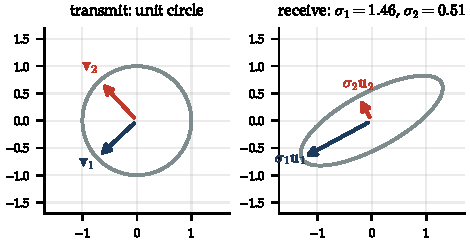
\includegraphics[width=0.62\linewidth]{figs/ch19_svd_pipes}\caption{The SVD in pictures. A $2\times2$ channel turns the circle of all unit
transmit vectors into an ellipse. The transmit directions $\vect{v}_1,\vect{v}_2$ land on the
ellipse's axes, stretched by $\sigma_1$ and $\sigma_2$: two private pipes, one wide and one
narrow.}\label{fig:ch19_svd_pipes}\end{figure}

Every complex matrix has a \term{singular value decomposition}
\begin{equation}
\vect{H}=\vect{U}\vect{\Sigma}\vect{V}^{\mathsf H},
\label{eq:ch19:svd}
\end{equation}
where $\vect{U}$ ($N_r\times N_r$) and $\vect{V}$ ($N_t\times N_t$) are unitary and $\vect{\Sigma}$
is $N_r\times N_t$ with the non-negative singular values $\sigma_1\ge\sigma_2\ge\dots\ge\sigma_m$,
$m=\operatorname{rank}\vect{H}\le\min(N_t,N_r)$, on its diagonal. The squares $\lambda_i=\sigma_i^2$
are the non-zero eigenvalues of $\vect{H}\vect{H}^{\mathsf H}$. Suppose the transmitter sends
$\vect{x}=\vect{V}\tilde{\vect{x}}$ and the receiver computes $\tilde{\vect{y}}=\vect{U}^{\mathsf H}\vect{y}$.
Then
\begin{equation}
\tilde{\vect{y}}=\vect{U}^{\mathsf H}\vect{U}\vect{\Sigma}\vect{V}^{\mathsf H}\vect{V}\tilde{\vect{x}}+\vect{U}^{\mathsf H}\vect{n}
=\vect{\Sigma}\tilde{\vect{x}}+\tilde{\vect{n}},
\qquad \tilde y_i=\sigma_i\tilde x_i+\tilde n_i,\quad i=1,\dots,m,
\label{eq:ch19:parallel}
\end{equation}
and, because $\vect{U}$ is unitary, $\tilde{\vect{n}}$ is still white with the same variance. The
MIMO channel has become $m$ independent scalar channels---\emph{eigenmodes} or
\emph{eigen-channels}---with power gains $\lambda_i$. No information is lost or created by the
unitary transformations, so the capacity of the MIMO channel equals the capacity of these parallel
channels. Geometrically: the columns of $\vect{V}$ are the directions in transmit space that the
channel maps onto orthogonal directions (the columns of $\vect{U}$) in receive space, stretched by
$\sigma_i$.

\subsection{Capacity with and without transmitter knowledge}

With a Gaussian input of covariance $\vect{Q}=\E[\vect{x}\vect{x}^{\mathsf H}]$, the mutual
information of~\eqref{eq:ch19:model} given $\vect{H}$ is
$\log_2\det(\vect{I}+\vect{H}\vect{Q}\vect{H}^{\mathsf H}/N_0)$, and capacity is its maximum over
$\vect{Q}$ subject to $\operatorname{tr}\vect{Q}\le E_s$. Two cases matter.

\emph{No CSIT.} A transmitter that does not know $\vect{H}$ cannot favour any direction, and for
the i.i.d.\ Rayleigh channel the optimal choice is $\vect{Q}=(E_s/N_t)\vect{I}$, giving
\begin{equation}
C=\log_2\det\Big(\vect{I}_{N_r}+\frac{\rho}{N_t}\vect{H}\vect{H}^{\mathsf H}\Big)
=\sum_{i=1}^m\log_2\Big(1+\frac{\rho}{N_t}\lambda_i\Big)\quad\text{b/s/Hz}.
\label{eq:ch19:capeq}
\end{equation}
This is \texttt{commlib.capacity\_equal\_power} and Equation~\eqref{eq:ch13:mimo}. In words: add up
Shannon's formula over the private pipes, each with its own SNR.

\emph{Full CSIT.} A transmitter that knows $\vect{H}$ sends along the eigenvectors, choosing
the input covariance $\vect{Q}=\vect{V}\operatorname{diag}(p_1,\dots,p_m)\vect{V}^{\mathsf H}$,
and allocates its power over the parallel channels~\eqref{eq:ch19:parallel} by
\term{water-filling}, exactly as in Section~\ref{sec:ch13:waterfill}: picture each pipe as a vessel
whose floor is raised by $N_0/\lambda_i$, and pour in the power until it all sits at one water level
$\mu$ (Figure~\ref{fig:ch19_waterfill_eig}):
\begin{equation}
p_i=\Big(\mu-\frac{N_0}{\lambda_i}\Big)^+,\quad \sum_ip_i=E_s,\qquad
C_{\text{WF}}=\sum_{i=1}^m\log_2\Big(1+\frac{p_i\lambda_i}{N_0}\Big).
\label{eq:ch19:capwf}
\end{equation}

This is \texttt{commlib.capacity\_waterfilling}. At high SNR the water is deep, all eigenmodes get
nearly equal power and the CSIT gain is small (for $4\times4$ i.i.d.\ Rayleigh at 20\,dB, 22.3 versus
22.1\,b/s/Hz). At low SNR water-filling puts all the power into the strongest eigenmode---pure
beamforming---and the gain is substantial: for a $4\times4$ channel at 0\,dB, 4.2 versus 3.4\,b/s/Hz,
a 25\% increase. Transmitter knowledge matters most exactly where cell-edge users live, and in
correlated channels where a few eigenmodes dominate.

\mdcfig[0.5]{ch19_cap_vs_n}{The $\min(N_t,N_r)$ law. Ergodic capacity of $N\times N$ i.i.d.\
Rayleigh links (solid) grows in a straight line with $N$; $1\times N$ links (dashed) gain only
array gain, a logarithm.}

\begin{tryit}[Pour water into the pipes]
In Lab~10, open \emph{Eigen-channels and water-filling}. Start at 4 transmit and 4 receive
antennas and drag \emph{SNR} from $-10$ to 30\,dB: watch the water level rise until it covers every
pipe, and the \emph{Water-filling gain} readout shrink towards zero. Then raise \emph{Antenna
correlation $\rho$} to 0.95: two pipes collapse to near-useless slivers, and water-filling's
advantage returns even at high SNR.
\end{tryit}

\subsection{Ergodic capacity and the $\min(N_t,N_r)$ law}

When the code spans many independent channel realisations (fast fading, or OFDM over a wide band),
the relevant figure is the \term{ergodic capacity} $\E_{\vect{H}}[C(\vect{H})]$. At high SNR each
term of~\eqref{eq:ch19:capeq} behaves like $\log_2\rho+\log_2(\lambda_i/N_t)$, so
\begin{equation}
C\approx\min(N_t,N_r)\log_2\rho+\text{constant},
\label{eq:ch19:slope}
\end{equation}
and capacity rises by $\min(N_t,N_r)$ bits per second per hertz for every 3\,dB of SNR. The
number $\min(N_t,N_r)$ is the number of \term{spatial degrees of freedom}, the \emph{pre-log
factor} or \emph{multiplexing gain}. Double the antennas at both ends and you double the capacity;
put them at only one end and you gain only a logarithm (Figure~\ref{fig:ch19_cap_vs_n}). At low
SNR, by contrast, $\log_2(1+x)\approx x\log_2e$ and
$C\approx(\rho/N_t)\,\E[\operatorname{tr}\vect{H}\vect{H}^{\mathsf H}]\log_2e=N_r\rho\log_2e$: receive
antennas help linearly through array gain, while transmit antennas help only if CSIT lets them
beamform. Figure~\ref{fig:ch19_capacity}(b) shows how these laws are bent by real channels:
correlation lowers the curves at practical SNRs, and the keyhole reduces the slope to one.

\mdcfig{ch19_capacity}{(a) Mean eigenvalues of $\vect{H}\vect{H}^{\mathsf H}$ for $4\times4$
channels: i.i.d.\ Rayleigh (navy), Kronecker exponential correlation with $\rho=0.7$ (green) and
$0.95$ (orange) at both ends, and a keyhole (red; its last three eigenvalues are zero). (b) Ergodic
capacity of the same channels without CSIT (solid), with water-filling for the i.i.d.\ case
(dotted), and of a single-antenna link. (c) Distribution of the capacity of i.i.d.\ Rayleigh
channels at 10\,dB; the dots mark the 10\% outage capacity. More antennas both raise and
\emph{steepen} the distribution.}

\begin{worked}[A $4\times4$ link at 20\,dB]
A $4\times4$ MIMO-OFDM link operates at an average SNR per receive antenna of 20\,dB in rich
scattering. Estimate its ergodic capacity, its 10\% outage capacity, and the effect of
correlation.

\emph{Ergodic.} Averaging~\eqref{eq:ch19:capeq} over 20\,000 i.i.d.\ Rayleigh draws gives
22.1\,b/s/Hz, compared with 5.9\,b/s/Hz for a $1\times1$ link at the same SNR: 3.8 times as much,
close to the factor 4 of~\eqref{eq:ch19:slope}. A quick check with the mean eigenvalues
(9.8, 4.4, 1.6 and 0.25 in linear terms), each scaled by $\rho/N_t=25$, gives
$\sum\log_2(1+25\lambda_i)=7.9+6.8+5.4+2.8=22.9$\,b/s/Hz; by Jensen's inequality this
overestimates the mean, as it does here, slightly.

\emph{Outage.} The 10\% outage capacity is 19.6\,b/s/Hz for $4\times4$ but only 3.5\,b/s/Hz for
$1\times1$, a ratio of more than five. In a slowly fading channel the multi-antenna link is
not only faster but far more \emph{reliable}: its capacity distribution is narrow because it
averages over 16 fading coefficients (Figure~\ref{fig:ch19_capacity}(c)).

\emph{Correlation.} With $\rho=0.7$ at both ends the ergodic capacity falls to 17.6\,b/s/Hz, and with
$\rho=0.95$ to 10.4\,b/s/Hz---less than a $2\times2$ i.i.d.\ link at the same SNR (11.4). A keyhole
gives 8.3\,b/s/Hz.

\emph{In practice.} Real receivers with finite constellations, imperfect channel estimates and
practical codes achieve a fraction of these figures. Four layers of 256-QAM at a code rate of about
0.9 carry about 29 coded-and-decoded bits per resource element before overheads, which is the
peak-rate regime of LTE-Advanced and NR handsets; reaching it requires SNRs in the high twenties
of decibels and a well-conditioned channel, which is why peak rates are demonstrated close to the
cell site.
\end{worked}

\subsection{Outage capacity}

\mdcpairany{ch19_paulraj}{Arogyaswami Paulraj, whose 1992 patent application with Thomas Kailath
proposed sending independent streams from several antennas and separating them at the
receiver.}{ch19_foschini}{Gerard Foschini of Bell Labs (photographed in 2009), whose BLAST
architecture and capacity analysis showed that capacity can grow in proportion to the number of
antennas.}

For a slowly fading channel and a delay-limited code that sees only one realisation of
$\vect{H}$, there is no ergodic averaging, and the meaningful quantity is the \term{outage
probability}
\begin{equation}
P_{\text{out}}(R)=P\big(C(\vect{H})<R\big),
\end{equation}
or its inverse, the $\epsilon$-outage capacity $C_\epsilon$, the rate supported by a fraction
$1-\epsilon$ of channels (Section~\ref{sec:ch13:fading}). Figure~\ref{fig:ch19_capacity}(c) shows
both effects of extra antennas: the median moves right (multiplexing) and the lower tail is pulled
in (diversity). The $1\times4$ curve is instructive. It averages four fading coefficients, as the
$2\times2$ channel does, so its tail is equally steep and its 10\% outage capacity is actually
slightly higher (4.2 against 3.9\,b/s/Hz at 10\,dB); but it has only one spatial degree of freedom,
so its median and its growth with SNR are lower. The precise way in which outage probability falls
with SNR, for a rate that itself grows with SNR, is the subject of Section~\ref{sec:ch19:dmt}.

\mdcfig{ch19_dmt}{(a) The optimal diversity--multiplexing trade-off of Zheng and Tse for several
antenna configurations. (b) Where practical schemes for a $2\times2$ channel sit: repetition coding
(full diversity, at most half a degree of freedom), Alamouti (full diversity, but a maximum
multiplexing gain of 1), V-BLAST with ML detection (full multiplexing, receive diversity only) and
V-BLAST with zero forcing (diversity one at best). Only carefully designed codes, such as the
Golden code, achieve the whole optimal curve.}

\begin{tryit}[Find the keyhole]
In Lab~10's \emph{Ergodic and outage capacity}, set 4 transmit and 4 receive antennas at 20\,dB and
read \emph{High-SNR slope}: close to four. Now switch \emph{Channel} to \emph{Keyhole}. The entries
are still uncorrelated, but the slope collapses to one---every stream is squeezing through the same
hole. Move \emph{Outage probability} to 1\% and compare \emph{Outage capacity $C_\varepsilon$} for
$1\times4$ and $2\times2$.
\end{tryit}

\begin{history}[Bell Labs, Stanford and the discovery of MIMO]
The capacity of multi-antenna links was found several times in the late 1980s and 1990s. Jack
Winters at Bell Labs analysed ``the capacity of radio communication systems with diversity in a
Rayleigh fading environment'' in 1987, showing that $N$ antennas at each end could support up to
$N$ channels in the same bandwidth. Arogyaswami Paulraj and Thomas Kailath at Stanford filed a
patent in 1992 (US~5,345,599, granted 1994) on sending separate data streams from multiple
antennas and separating them at the receiver---often cited as the first explicit proposal of
spatial multiplexing. Gerard Foschini at Bell Labs published the diagonally layered space--time
architecture (D-BLAST) in the \emph{Bell Labs Technical Journal} in 1996, and with Michael Gans the
capacity analysis ``On limits of wireless communications in a fading environment when using
multiple antennas'' (1998), which showed the linear growth with $\min(N_t,N_r)$. Independently,
\.{I}.~Emre Telatar, also at Bell Labs, derived the capacity and the water-filling solution
rigorously in a 1995 technical memorandum, published in 1999 as ``Capacity of multi-antenna
Gaussian channels''. In 1998 Wolniansky, Foschini, Golden and Valenzuela reported a laboratory
prototype of the simpler vertical architecture, V-BLAST, which achieved spectral efficiencies of
20--40\,b/s/Hz indoors with 8 transmit and 12 receive antennas---an order of magnitude beyond any
deployed system of the day. Within ten years, MIMO was in every new Wi-Fi and cellular standard.
\end{history}

%======================================================================
\section{The diversity--multiplexing trade-off}
\label{sec:ch19:dmt}
%======================================================================

A MIMO channel offers both diversity (up to $N_tN_r$, from the $N_tN_r$ fading coefficients) and
multiplexing (up to $\min(N_t,N_r)$ streams). Alamouti's code takes all the diversity of a
$2\times2$ channel and only one stream; V-BLAST takes two streams and, with a linear receiver, very
little diversity. Can one have both at once? It is the old engineering bargain between going fast
and going safely, and Lizhong Zheng and David Tse answered it in 2003 with a single curve.

\mdcfig[0.5]{ch19_dmt_outage}{The trade-off measured. Outage probability of a $2\times2$ i.i.d.\
channel whose rate grows as $r\log_2\rho$, simulated over 400\,000 channels. The higher the
multiplexing gain $r$, the shallower the slope, as $d^*(r)$ predicts: about 2.5, 1 and 0.5
decades per 10\,dB.}

Consider a family of codes whose rate grows with SNR as $R(\rho)=r\log_2\rho$; the number $r$
is the \term{multiplexing gain}, the number of degrees of freedom being used. The
\emph{diversity gain} of the family is the slope of its error probability,
$d=-\lim_{\rho\to\infty}\log P_e/\log\rho$. Zheng and Tse showed that for the i.i.d.\ Rayleigh channel
with a block length $T\ge N_t+N_r-1$, the best achievable diversity at multiplexing gain $r$ is the
piecewise-linear curve $d^*(r)$ joining the points
\begin{equation}
\big(k,\;(N_t-k)(N_r-k)\big),\qquad k=0,1,\dots,\min(N_t,N_r).
\label{eq:ch19:dmt}
\end{equation}
At $r=0$ (a fixed rate) the full diversity $N_tN_r$ is available; at $r=\min(N_t,N_r)$ (all
degrees of freedom used) none is left. Every integer step in multiplexing costs diversity, as if
using one spatial dimension for data removed one transmit and one receive antenna from the
diversity count (Figure~\ref{fig:ch19_dmt}(a)).

The intuition comes from outage. At high SNR, an outage at rate $r\log_2\rho$ happens when too
many of the eigenvalues $\lambda_i$ are small---of order $\rho^{-1}$ instead of order one---for the
remaining ones to carry the rate. Asking for $k$ eigenvalues to collapse is like asking a random
matrix to lose $k$ dimensions, and the probability of that event scales as
$\rho^{-(N_t-k)(N_r-k)}$ (Figure~\ref{fig:ch19_dmt_outage}).

The DMT gives a common yardstick for space--time schemes (Figure~\ref{fig:ch19_dmt}(b)). The
Alamouti code with two receive antennas achieves $d(r)=4(1-r)$: optimal at $r=0$ but unable to
exceed one degree of freedom. V-BLAST with joint ML detection achieves $N_r(1-r/N_t)$, optimal at
full multiplexing but with only receive diversity at low rates; with zero forcing it achieves
$(N_r-N_t+1)(1-r/N_t)$, which for a square system is diversity one. The Golden code and other
codes built from cyclic division algebras with the \emph{non-vanishing determinant} property
achieve the entire optimal curve.

\mdcfig[0.62]{ch19_zf_geometry}{Zero forcing as geometry. To recover stream 1, ZF listens along the
dashed red direction, orthogonal to $\vect{h}_2$. Only the projection of $\vect{h}_1$ on that
direction (thick red) survives. When the columns are well separated (left) little is lost; when
they are nearly parallel (right) the surviving signal is tiny and the noise is amplified about
fifteen-fold.}

\begin{keyidea}[Diversity and multiplexing are two uses of the same resource]
A MIMO channel's randomness can be spent on reliability or on rate. Rate increases that grow with
$\log\rho$ consume diversity; reliability gains at fixed rate consume none. In a modern system
the balance is set dynamically: link adaptation chooses the number of layers (the rank) and the
modulation and coding for each user every millisecond, using more streams when the channel is
strong and well conditioned and falling back to one beamformed stream (maximum diversity and array
gain) at the cell edge. The DMT is the theory behind that rank adaptation.
\end{keyidea}

\mdcfig[0.5]{ch19_zf_snr}{Spare antennas buy back diversity. Distribution of the post-ZF gain of
one of four streams, for 4, 5, 6 and 8 receive antennas (40\,000 i.i.d.\ channels each). With
$N_r=N_t$ the deep-fade tail has slope one; each extra receive antenna steepens it by one.}

\begin{tryit}[Measure a diversity slope]
In Lab~10's \emph{The diversity--multiplexing trade-off}, pick a $2\times2$ channel and drag
\emph{Multiplexing gain r} from 0.3 towards 1.9. The \emph{Measured outage slope} readout falls
along the piecewise-linear curve: the faster you insist on going, the fewer decades of reliability
each 10\,dB buys.
\end{tryit}

%======================================================================
\section{Receivers for spatial multiplexing}
\label{sec:ch19:detection}
%======================================================================

In spatial multiplexing (V-BLAST, or ``open-loop'' MIMO), $N_t$ independent streams are sent from
$N_t$ antennas and the receiver must separate them from $N_r\ge N_t$ observations
$\vect{y}=\vect{H}\vect{x}+\vect{n}$---the party again, with the listener trying to follow every
speaker at once. This is a small linear inverse problem with discrete unknowns, and it is exactly
the problem of Chapter~\ref{ch:equalization} with space playing the role of time: the columns of
$\vect{H}$ interfere with each other as the taps of a dispersive channel do. The same family of
solutions appears---linear zero-forcing and MMSE, decision feedback, and maximum
likelihood---with the same trade-offs between noise enhancement, error propagation and
complexity.

\subsection{Zero forcing}

The \term{zero-forcing} (ZF) receiver inverts the channel,
\begin{equation}
\hat{\vect{x}}_{\text{ZF}}=\vect{H}^{+}\vect{y}=(\vect{H}^{\mathsf H}\vect{H})^{-1}\vect{H}^{\mathsf H}\vect{y}
=\vect{x}+(\vect{H}^{\mathsf H}\vect{H})^{-1}\vect{H}^{\mathsf H}\vect{n},
\end{equation}
which removes all inter-stream interference and leaves noise whose variance on stream $k$ is
$N_0[(\vect{H}^{\mathsf H}\vect{H})^{-1}]_{kk}$. When $\vect{H}$ is ill-conditioned this is large:
inverting a small singular value amplifies the noise, exactly the noise enhancement of a ZF
equaliser near a spectral null (Section~\ref{sec:ch12:zf}). Geometrically, the ZF filter for stream
$k$ projects $\vect{y}$ onto the part of $\vect{h}_k$ orthogonal to all the other columns
(Figure~\ref{fig:ch19_zf_geometry}); it spends $N_t-1$ of the receiver's $N_r$ dimensions on
nulling, and only $N_r-N_t+1$ remain for diversity. For i.i.d.\ Rayleigh $\vect{H}$, the post-ZF
SNR of each stream is chi-square with $2(N_r-N_t+1)$ degrees of freedom, so the diversity order is
$N_r-N_t+1$: one for a square system (Figure~\ref{fig:ch19_zf_snr}). This is
\texttt{commlib.zf\_detect}.

\subsection{Linear MMSE}

The \term{MMSE receiver} minimises $\E\|\hat{\vect{x}}-\vect{x}\|^2$ and balances interference
against noise---it is willing to let a little interference through if that avoids blowing up the
noise:
\begin{equation}
\vect{W}_{\text{MMSE}}=\Big(\vect{H}^{\mathsf H}\vect{H}+\frac{N_0}{E_x}\vect{I}\Big)^{-1}\vect{H}^{\mathsf H},
\qquad
\text{SINR}_k=\frac{1}{\big[(\vect{I}+\tfrac{E_x}{N_0}\vect{H}^{\mathsf H}\vect{H})^{-1}\big]_{kk}}-1,
\label{eq:ch19:mmse}
\end{equation}
with $E_x$ the energy per stream. At high SNR it converges to ZF; at low SNR it converges to MRC
on each stream (the matched filter $\vect{H}^{\mathsf H}$). It is never worse than ZF and is
\texttt{commlib.mmse\_detect}. Like the MMSE equaliser, the raw output is biased towards zero and
must be rescaled before slicing a QAM constellation (Section~\ref{sec:ch12:bias}). Its diversity
order is the same as ZF's for uncoded transmission at fixed rate, but its coding gain is better
(Figure~\ref{fig:ch19_detector_constellations}) and, with a channel code across many channel
realisations, the difference is substantial.

\mdcfig[0.62]{ch19_detector_constellations}{Stream 1 of a badly conditioned $2\times2$ QPSK channel
at 20\,dB, after zero forcing (left) and after unbiased MMSE (right). ZF's noise enhancement smears
the four points into one cloud; MMSE trades a little residual interference for much less noise and
halves the symbol error rate.}

\subsection{Successive interference cancellation and V-BLAST ordering}

The decision-feedback idea carries over directly. Detect one stream, subtract its contribution
from $\vect{y}$, and detect the next stream from a problem with one fewer unknown, which now has
one more dimension available for diversity. It is how you follow a conversation at a party: catch
the loudest voice first, mentally ``subtract'' it, and the quieter ones become easier to hear. The
order matters: with errors propagating forward, the first decision should be the most reliable one.
The V-BLAST algorithm of Wolniansky, Foschini, Golden and Valenzuela (1998) chooses, at each stage,
the remaining stream with the largest post-detection SNR, which for ZF nulling is the one with the
smallest row norm of the pseudo-inverse. With MMSE filters instead of ZF and the same ordering, this
is \term{MMSE-SIC}, the \texttt{commlib.mmse\_sic\_detect} function: at each step it picks the stream
with the smallest MMSE (the diagonal of $(\vect{I}+\vect{H}_r^{\mathsf H}\vect{H}_r/N_0)^{-1}$),
slices it, and subtracts.

MMSE-SIC has a remarkable property. If each stream carries a capacity-achieving Gaussian code at a
rate matched to its own post-cancellation SINR and the decoded (not merely sliced) streams are
cancelled, the sum of the stream rates equals the MIMO capacity~\eqref{eq:ch19:capeq} exactly. This
follows from the chain rule of mutual information: $\log\det(\vect{I}+\rho/N_t\,\vect{H}\vect{H}^{\mathsf H})$
splits into a sum of per-stream terms, one for each stage of cancellation. MMSE-SIC is therefore
not a heuristic but an information-theoretically optimal architecture, a fact that underlies both
the uplink of multi-user systems (Section~\ref{sec:ch19:mumimo}) and the layered designs of
Foschini. Its weaknesses are practical: per-stream rate control, latency (each stage waits for the
previous decoder), and error propagation if a decoded stream is wrong.

\subsection{Maximum likelihood and the sphere decoder}

The optimal detector for equiprobable vectors is
\begin{equation}
\hat{\vect{x}}_{\text{ML}}=\arg\min_{\vect{x}\in\mathcal{A}^{N_t}}\|\vect{y}-\vect{H}\vect{x}\|^2,
\label{eq:ch19:ml}
\end{equation}
which achieves the full receive diversity $N_r$ for each stream and the best coding gain. A
brute-force search over all $M^{N_t}$ candidate vectors (\texttt{commlib.ml\_detect}) is easy for
$2\times2$ QPSK (16 candidates), plausible for $4\times4$ QPSK (256), and hopeless for $4\times4$
64-QAM (about 16.8 million per subcarrier per symbol). Figure~\ref{fig:ch19_detectors}(a) shows what
is at stake for $4\times4$ QPSK: at a symbol error rate of $10^{-3}$ ML needs about 16\,dB,
MMSE-SIC about 20\,dB, and ZF and MMSE more than 30\,dB.

\mdcfig{ch19_detectors}{(a) Symbol error rate of $4\times4$ spatial multiplexing with QPSK over
i.i.d.\ Rayleigh fading, for the four detectors in \texttt{commlib}. ZF and MMSE have diversity
order one; ordered MMSE-SIC does better; ML has diversity order four and is more than 15\,dB
ahead of ZF at $10^{-3}$. (b) Complexity of a Schnorr--Euchner sphere decoder for $4\times4$ 16-QAM (an
eight-level real tree with four branches per node), counted as tree nodes visited. At high SNR
the sphere decoder visits barely more nodes than SIC; at low SNR, and in its worst cases, it
visits many more. The fixed-complexity K-best detector and the full ML tree are shown for
comparison.}

The \term{sphere decoder} finds the ML solution without visiting all candidates. Think of a
treasure hunt in a tree of rooms: the deeper you go, the more it has cost you to get there, so once
you have found \emph{one} treasure you never need to enter a room whose entry fee already exceeds
it. Take the QR decomposition $\vect{H}=\vect{Q}\vect{R}$, with $\vect{R}$ upper triangular, and let
$\vect{z}=\vect{Q}^{\mathsf H}\vect{y}$. Then
\begin{equation}
\|\vect{y}-\vect{H}\vect{x}\|^2=\|\vect{z}-\vect{R}\vect{x}\|^2+\text{const}
=\sum_{i=1}^{N_t}\Big|z_i-\sum_{j\ge i}R_{ij}x_j\Big|^2+\text{const}.
\end{equation}
The term for $i=N_t$ depends only on $x_{N_t}$; the term for $i=N_t-1$ on $x_{N_t-1}$ and
$x_{N_t}$; and so on. The search is a tree whose root chooses $x_{N_t}$, whose second level chooses
$x_{N_t-1}$, and whose leaves are complete vectors, with each partial path carrying a partial
distance that can only grow as one descends (Figure~\ref{fig:ch19_sphere_tree}). A depth-first search
that keeps the best complete distance found so far as a radius, and prunes any branch whose partial
distance already exceeds it, finds the ML solution while visiting a small fraction of the tree.
Visiting the children of each node in order of increasing distance (the \emph{Schnorr--Euchner}
enumeration) finds a good leaf quickly---the first leaf reached is the SIC solution---and shrinks
the radius fast. The idea of enumerating lattice points inside a sphere goes back to Fincke and
Pohst (1985); Viterbo and Boutros brought it to fading channels in 1999 and Damen, Chkeif and
Belfiore to space--time detection in 2000.

\mdcfig{ch19_sphere_tree}{A real sphere-decoder run on a three-level tree with four amplitude
levels per level (84 nodes in all). Navy: the nodes the Schnorr--Euchner search actually visited;
grey: the parts of the tree it proved could not contain the answer and never entered; red: the
maximum-likelihood path it returns.}

The sphere decoder's catch is that its complexity is a random variable
(Figure~\ref{fig:ch19_detectors}(b)). At high SNR it visits barely more nodes than SIC, but at low SNR
or for badly conditioned channels the radius stays large and the search wanders; its expected
complexity is still exponential in $N_t$, only with a much smaller exponent. Hardware needs a fixed
throughput, so practical chips use breadth-first variants. The \term{K-best} detector keeps the $K$
best partial paths at each level and extends only those, giving a fixed, pipelinable workload of
roughly $KM$ distance computations per level and near-ML performance for $K$ of 8--32 at
moderate constellation sizes; the \emph{fixed-complexity sphere decoder} enumerates all values of
the first one or two symbols and then runs SIC. Lattice-reduction-aided detection changes the basis
of the lattice so that a simple linear or SIC detector achieves full diversity.

\begin{tryit}[Race the detectors]
Open Lab~10's \emph{ZF, MMSE, SIC and ML}, choose \emph{Configuration} \emph{4$\times$4, QPSK} and
\emph{Effort} \emph{Thorough}, and press \emph{Run again}. Watch the four curves fill in: ZF and MMSE
share the shallow single-antenna slope, ML plunges. Switch to \emph{2$\times$4, QPSK}: with two spare
receive antennas even ZF gains diversity $N_r-N_t+1=3$.
\end{tryit}

\subsection{Soft-output detection}

A modern MIMO receiver never feeds hard decisions to its LDPC or turbo decoder; it feeds
log-likelihood ratios for every coded bit. For bit $b$ of the label of $\vect{x}$, the max-log
approximation is
\begin{equation}
L(b)\approx\frac{1}{N_0}\Big(\min_{\vect{x}:\,b=1}\|\vect{y}-\vect{H}\vect{x}\|^2-\min_{\vect{x}:\,b=0}\|\vect{y}-\vect{H}\vect{x}\|^2\Big),
\end{equation}
so a soft-output ML detector must find, for each bit, the best candidate with that bit equal to 0
and the best with it equal to 1 (Figure~\ref{fig:ch19_llr}). The \emph{list sphere decoder} of Hochwald and ten Brink (2003)
keeps a list of good candidates from the tree search and computes the LLRs over the list;
soft-output K-best detectors do the same with their survivor lists. Linear MMSE detectors produce
LLRs very cheaply from the per-stream SINR~\eqref{eq:ch19:mmse}, treating residual interference as
Gaussian noise; this is the workhorse in handsets. At the high end, \emph{iterative detection and
decoding} feeds the decoder's extrinsic information back to the detector, which cancels the
interference it now believes it knows, in exactly the turbo-equalisation loop of
Section~\ref{sec:ch12:turbo}.

\mdcfig[0.5]{ch19_llr}{Soft output in action: max-log LLRs of one bit from a $2\times2$ QPSK
ML detector at 10\,dB, over 6000 random channels. Most bits come out confidently right; the
uncertain ones cluster near zero, and the channel decoder that receives these numbers knows to
distrust them.}

\begin{inpractice}[What is inside a MIMO receiver chip]
A Wi-Fi 6 client with two antennas and a 160\,MHz channel must detect two streams of up to
1024-QAM on nearly two thousand subcarriers every 13.6\,$\mu$s, and an access point receiving uplink
MU-MIMO must do it for several stations at once. Base-station and access-point modems typically
implement MMSE detection with LLR computation as the baseline and add near-ML detectors (K-best or
sphere-decoder variants) for the high-order, low-rank cases where they help most. Handset modems
for LTE and NR use MMSE-IRC as the default and, in some designs, near-ML detection for two-layer
reception. Because channel estimates come from pilots, every detector is fed an estimate
$\hat{\vect{H}}$ rather than $\vect{H}$, and with dense constellations it is often the estimation
error, not the detector's sub-optimality, that limits throughput: a 1024-QAM stream needs an
SNR after detection in the mid-thirties of decibels, so the channel estimate must be correspondingly
accurate.
\end{inpractice}

\mdcfig[0.5]{ch19_eigbf}{Eigen-beamforming on a $4\times4$ i.i.d.\ channel (navy) against
four-branch MRC (orange) and a single antenna pair (grey), 20\,000 channel draws. Eigen-beamforming
gains almost 10\,dB on average, and its distribution has a far thinner low tail: diversity order 16
instead of 4.}

%======================================================================
\section{Precoding with channel knowledge at the transmitter}
\label{sec:ch19:precoding}
%======================================================================

The receiver-side techniques above need no CSIT. A transmitter that knows the channel can do
better: send along the eigenmodes (Section~\ref{sec:ch19:capacity}), choose the number of streams,
avoid weak directions entirely and, with many users, separate them in space. The difficulty is
practical: the channel is measured at the receiver, and getting it to the transmitter costs
either feedback overhead (in FDD, where uplink and downlink use different frequencies) or relies
on reciprocity (in TDD, where they share one). It is like a photographer who cannot see the
subject and must be told by an assistant where to point the camera: the better and quicker the
description, the sharper the picture. This section covers the single-user case and the feedback
machinery of LTE and NR; reciprocity is taken up with massive MIMO.

\subsection{SVD precoding}

With perfect CSIT, the transmitter sends $\vect{x}=\vect{V}_{N_s}\vect{P}^{1/2}\vect{s}$, where
$\vect{V}_{N_s}$ holds the first $N_s$ right singular vectors and $\vect{P}$ the water-filling
powers, and the receiver applies $\vect{U}_{N_s}^{\mathsf H}$. The streams arrive on separate
eigenmodes with no interference between them~\eqref{eq:ch19:parallel}, each with its own SNR
$p_i\lambda_i/N_0$, and each can use its own modulation and code rate. With $N_s=1$ this is
\term{eigen-beamforming}, the MIMO generalisation of MRT: the transmitter sends along $\vect{v}_1$
and the receiver combines along $\vect{u}_1$, giving SNR $\lambda_1E_s/N_0$ with
$\E[\lambda_1]$ between $\max(N_t,N_r)$ and $N_tN_r$. Eigen-beamforming over a $4\times4$ i.i.d.\
channel collects an average of about 9.8 (9.9\,dB) instead of the 4 of four-branch MRC and achieves
the full diversity order 16.

\subsection{Codebook-based precoding: PMI, RI and CQI}

\mdcfig[0.48]{ch19_codebook_polar}{LTE's two-port rank-one codebook seen as beams. With two antennas
half a wavelength apart, the four phase choices $\phi$ point energy broadside, to either side, or
into two end-fire lobes. Two bits of feedback pick the best one.}

In FDD systems the base station cannot measure the downlink channel, and sending back the full
$\vect{H}$ for every subband is too expensive. LTE's solution, inherited by NR, is a
\term{codebook}: a finite set of precoding matrices known to both ends---a menu from which the
handset orders by number. The handset measures the channel from reference signals, chooses the
best matrix, and reports its index. The channel state information (CSI) report has three main
parts:
\begin{itemize}
\item the \term{rank indicator} (RI), the number of layers the handset recommends;
\item the \term{precoding matrix indicator} (PMI), the index of the recommended precoder for that
rank, wideband or per subband;
\item the \term{channel quality indicator} (CQI), a 4-bit index into a table of modulation and
coding schemes, giving the highest rate the handset expects to decode with a block error rate of
about 10\% if the recommended precoder and rank are used.
\end{itemize}
The base station is free to ignore the recommendation---for example, to pair users for MU-MIMO---but
the CQI it receives was computed for the recommended precoder. For two antenna ports, LTE's rank-one
codebook is the four vectors $\frac{1}{\sqrt2}[1,\;e^{j\phi}]^{\mathsf T}$ with
$\phi\in\{0,\pi/2,\pi,3\pi/2\}$: choose the relative phase that makes the two antennas add best at
the handset, quantised to two bits. With two half-wavelength-spaced antennas these four choices
look like four beams (Figure~\ref{fig:ch19_codebook_polar}). For four ports, Release~8 used sixteen
Householder matrices; for eight ports, Release~10 introduced the \emph{dual-stage} structure
$\vect{W}=\vect{W}_1\vect{W}_2$ that NR generalised.

\mdcfig{ch19_codebook}{(a) The NR Type I DFT codebook for a four-column array with oversampling
$O_1=4$: sixteen beams (grey), of which every fourth (dark) forms an orthogonal set. Oversampling
fills in the gaps between orthogonal beams. (b) Limited feedback: average beamforming gain
$N_t\,\E|\vect{h}^{\mathsf H}\vect{w}|^2/\|\vect{h}\|^2$ achieved by the best of $2^B$ random unit
vectors (random vector quantisation), against the feedback bits $B$, compared with perfect CSIT
(dashed). With few antennas a few bits suffice; with many, the bits required grow in proportion to
$N_t-1$.}

\subsection{NR Type I and Type II CSI}

An NR base station with a two-dimensional cross-polarised panel of $N_1\times N_2$ dual-polarised
elements (up to 32 CSI-RS ports) uses a codebook built from DFT beams (TS~38.214):
\begin{itemize}
\item \textbf{Type I single-panel}: $\vect{W}_1$ selects one (or, for higher ranks, a few) beams from
a grid of two-dimensional DFT vectors oversampled by $O_1=O_2=4$, the same beam on both
polarisations; $\vect{W}_2$ selects a co-phasing factor between the polarisations from
$\{1,j,-1,-j\}$. Figure~\ref{fig:ch19_codebook}(a) shows the oversampled beam grid for a
four-column array: sixteen beams instead of the four orthogonal ones, so that any direction is
within about 1\,dB of a beam peak. Type I supports up to eight layers with modest feedback (tens of bits).
\item \textbf{Type II}: the handset reports a \emph{linear combination} of $L=2$, 3 or 4 orthogonal
DFT beams per polarisation, with an amplitude and a phase (QPSK or 8-PSK) for each beam,
polarisation and subband. This describes a multipath channel far better than a single beam and is
designed for MU-MIMO, where precise knowledge of each user's channel determines how well the base
station can null inter-user interference. Release~15 Type II supports up to two layers and its
reports can run to several hundred bits; the \emph{enhanced} Type II of Release~16 compresses the
per-subband coefficients with a DFT basis across frequency, reducing the overhead substantially and
supporting up to four layers, and later releases added port-selection variants for TDD-assisted
operation and Doppler-domain compression for moving users.
\end{itemize}
In plain words: Type~I says ``point roughly that way''; Type~II says ``it's mostly that way, a
bit of this other way, and a dash of a third, with these phases''. The first is enough for one
user; the second is what lets the base station squeeze several users into the same resources.

\subsection{How many bits of feedback?}

The theory of \emph{limited feedback} (Love, Heath and Strohmer; Mukkavilli, Sabharwal, Erkip and
Aazhang; both 2003) asks how close a $B$-bit codebook can come to perfect CSIT. For beamforming
in i.i.d.\ Rayleigh fading the best codebooks are \emph{Grassmannian line packings}, sets of
lines through the origin with the largest minimum angle between them. Random codebooks do almost as
well and are easier to analyse: the expected loss in beamforming gain decays roughly as
$2^{-B/(N_t-1)}$. Every extra antenna therefore needs roughly one more bit (for each halving of
the residual loss) to keep the same quality (Figure~\ref{fig:ch19_codebook}(b)). For single-user
beamforming a few bits per antenna are enough, because a small error in the beam direction costs
little gain. For multi-user MIMO the story is harsher: residual inter-user interference grows with
transmit power, so Jindal (2006) showed that to keep the rate loss bounded the feedback must grow
linearly with SNR in decibels, about $(N_t-1)/3$ bits per 1\,dB. This is the theoretical reason for
NR's elaborate Type II CSI, and a key argument for TDD reciprocity in massive MIMO.

\begin{table}[htbp]\centering\small
\caption{Multi-antenna features of some major standards (maximum values in the specifications;
deployed products often support fewer).}
\label{tab:ch19:standards}
\begin{tabularx}{\linewidth}{@{}l c >{\raggedright\arraybackslash}X >{\raggedright\arraybackslash}X@{}}
\toprule
Standard & Max.\ streams & Transmit diversity / beamforming & MU-MIMO and CSI\\
\midrule
WCDMA (Rel-99, Rel-7) & 2 (HSPA+ MIMO) & STTD (Alamouti), closed-loop phase feedback & --\\
802.11n (2009) & 4 & STBC, CDD, explicit/implicit beamforming & --\\
802.11ac (2013) & 8 & standardised NDP sounding, compressed beamforming report & DL MU-MIMO, up to 4 users\\
802.11ax (2021) & 8 & as 802.11ac & DL and UL MU-MIMO, with OFDMA\\
LTE Rel-8 (2008) & 4 DL, 1 UL & SFBC, SFBC-FSTD, large-delay CDD & codebook PMI/RI/CQI, 2 and 4 ports\\
LTE Rel-10 to 14 & 8 DL, 4 UL & dual-stage codebook, beamformed CSI-RS & MU-MIMO, FD-MIMO (up to 32 ports)\\
NR Rel-15 onward & 8 DL, 4 UL & beam management, SRS-based (reciprocity) precoding & Type I/II CSI, up to 32 CSI-RS ports, 12 or more orthogonal DM-RS ports\\
\bottomrule
\end{tabularx}
\end{table}

\begin{pitfall}[The precoder the handset assumed is not the precoder you used]
In codebook-based systems the CQI is computed for the handset's preferred precoder, single-user,
with no interference from co-scheduled users. When the scheduler pairs the handset with another
for MU-MIMO, or overrides its PMI, the actual SINR can be several decibels lower than the CQI
implies, and the first transmissions fail. Base stations therefore run an \emph{outer loop} that
adjusts an offset on the reported CQI to hold the observed block error rate near the target
(typically 10\%; Figure~\ref{fig:ch19_olla}). A badly tuned outer loop, or one that does not
distinguish single-user from multi-user transmissions, can quietly cost more throughput than any
detector improvement gains.
\end{pitfall}

\mdcfig[0.5]{ch19_olla}{An outer loop at work (simulation). The reported CQI is 4\,dB too
optimistic because of MU-MIMO pairing. Each failed block raises the back-off by 0.5\,dB, each
success lowers it by a ninth of that; within about fifty blocks the back-off settles at about 4--6\,dB
and the block error rate (orange) hovers around the 10\% target.}

%======================================================================
\section{Antenna arrays and beamforming}
\label{sec:ch19:arrays}
%======================================================================

Have you ever seen a stadium do the wave? Nobody runs anywhere. Each person simply stands up a
moment after the neighbour on their left, and a crest of motion sweeps around the ground at
hundreds of kilometres per hour. Change the delay between neighbours and the wave goes faster or
slower; reverse it and the wave turns around. A phased array works the same way. The matrix view of
MIMO treats antennas as abstract branches. Now consider geometry. When antennas are spaced
regularly and the propagation is dominated by a few directions---always true for line-of-sight
links, and approximately true for an elevated base station or a millimetre-wave link with few
clusters---the channel vector has a structure determined by the angle of arrival, and array
processing becomes \emph{spatial filtering}: shaping a pattern in angle, as a digital filter
shapes a response in frequency.

\mdcpairany{ch19_laola}{Fans doing ``the wave'' at a 2005 Confederations Cup match. Each person rises
a moment after their neighbour; the timing, not anyone's motion, sends the crest around the
stadium.}{ch19_wave_beam}{The array version. Top: eight elements fire the same carrier, each a
quarter-cycle later than the one below (red dots mark the crests). Bottom: that timing tilts the beam
of the eight-element array from broadside (grey) to $30^\circ$ (navy).}

\begin{analogy}[A stadium crowd doing the wave]
Each antenna in a phased array radiates the same signal, just delayed a little more than its
neighbour. Where those delayed copies arrive in step, they add up; everywhere else they partly
cancel. So the \emph{timing} across the crowd, not the strength of any one person, decides which
way the energy goes (Figure~\ref{fig:ch19_wave_beam}). The limits: a real crowd's wave moves along
the stands, whereas an array's ``wave'' points energy out into space; and the array uses a fixed
\emph{phase} step, which equals the right time delay only at one frequency---the root of beam squint
below.
\end{analogy}

\subsection{Steering vectors}

Consider a uniform linear array (ULA) of $N$ elements spaced $d$ apart, receiving a narrowband plane
wave from angle $\theta$ measured from broadside (Figure~\ref{fig:ch19_ula}). The wave reaches element
$n$ later than element 0 by $nd\sin\theta/c$, a phase lag of $2\pi nd\sin\theta/\lambda$. The vector
of complex gains across the array is the \term{steering vector}
\begin{equation}
\vect{a}(\theta)=\Big[1,\;e^{-j2\pi\frac{d}{\lambda}\sin\theta},\;e^{-j2\pi\frac{2d}{\lambda}\sin\theta},\;\dots,\;e^{-j2\pi\frac{(N-1)d}{\lambda}\sin\theta}\Big]^{\mathsf T},
\label{eq:ch19:steer}
\end{equation}
which is \texttt{commlib.ula\_steering}. It is a complex sinusoid in the element index with
\emph{spatial frequency} $u=(d/\lambda)\sin\theta$ cycles per element. The analogy with time-domain
signal processing is exact: the array samples the wavefront in space, $d$ is the sampling interval,
and $u$ plays the role of the normalised frequency $f/f_s$.

\begin{figure}[htbp]\centering
\begin{tikzpicture}[>=Stealth,font=\sffamily\scriptsize]
\foreach \n in {0,...,5}{
  \fill[navy] (\n*1.1,0) circle (0.09);
  \node[below=3pt] at (\n*1.1,0) {$\n$};
}
\node[below=3pt] at (6.6,0) {$\cdots\;N{-}1$};
\draw[navy,thick] (-0.3,0) -- (6.0,0);
\draw[<->] (0,-0.62) -- node[below]{$d$} (1.1,-0.62);
\def\th{30}
\foreach \s in {0,1,2}{
  \draw[accent,thick] ($(5.5,0)+({\th+90}:-0.2)+({90+\th}:0)+({\th}:\s*0.9+1.2)$) -- ++({\th+90}:3.6);
}
\draw[->,accent,very thick] ($(4.2,2.9)$) -- ++({180+\th}:1.1) node[midway,above left=-1pt]{plane wave};
\draw[dashed,gray] (0,0) -- (0,2.4);
\draw[gray] (0,0) -- ({90-\th}:2.4);
\draw[->,gray] (0,1.5) arc (90:{90-\th}:1.5) node[midway,above]{$\theta$};
\draw[navy,dashed] (1.1,0) -- ($(1.1,0)+({\th}:0.55)$);
\node[navy,align=left] at (2.55,0.75) {extra path\\$d\sin\theta$};
\node[navy,draw=navy,fill=navy!6,rounded corners,align=left] at (9.4,1.3)
 {$\vect{a}(\theta)=\big[1,\,e^{-j\psi},\,e^{-j2\psi},\dots\big]^{\mathsf T}$\\[2pt]
  $\psi=2\pi\frac{d}{\lambda}\sin\theta$\\[3pt]
  output $z=\vect{w}^{\mathsf H}\vect{y}$};
\end{tikzpicture}
\caption{A uniform linear array receiving a plane wave from angle $\theta$ off broadside. Each
element is $d\sin\theta$ further along the propagation path than its neighbour, so the signals
across the array form a linear phase progression---the steering vector---whose spatial frequency
encodes the direction. A beamformer weights and sums the element signals.}
\label{fig:ch19_ula}
\end{figure}

\subsection{The array factor, gain and beamwidth}

A beamformer with weights $\vect{w}$ produces $z=\vect{w}^{\mathsf H}\vect{y}$, and its response to a
plane wave from $\theta$ is the \term{array factor} $\mathrm{AF}(\theta)=\vect{w}^{\mathsf H}\vect{a}(\theta)$;
the full radiation pattern is the array factor times the element pattern. To point the beam at
$\theta_0$, choose $\vect{w}=\vect{a}(\theta_0)/\sqrt{N}$, the spatial matched filter. Summing the
geometric series gives the familiar Dirichlet kernel,
\begin{equation}
|\mathrm{AF}(\theta)|^2=\frac{1}{N}\left|\frac{\sin(N\psi/2)}{\sin(\psi/2)}\right|^2,
\qquad\psi=2\pi\frac{d}{\lambda}(\sin\theta-\sin\theta_0),
\label{eq:ch19:af}
\end{equation}
which peaks at $N$ for $\theta=\theta_0$. Several facts follow, each with a time-domain twin:
\begin{itemize}
\item \textbf{Array gain.} On receive, coherent combining raises the SNR by $N$
($10\log_{10}N$\,dB) over one element, whatever the direction, provided the beam points at the
source. On transmit, an array of $N$ elements each fed with power $P_e$ radiates $NP_e$ in total
and concentrates it with directivity gain $N$, so the EIRP is $N^2P_eG_e$: $20\log_{10}N$\,dB above
a single element. That quadratic law is why phased arrays with many small amplifiers are so
attractive at millimetre waves.
\item \textbf{Beamwidth.} The half-power beamwidth of a uniformly weighted array is
\begin{equation}
\theta_{3\,\text{dB}}\approx\frac{0.886\,\lambda}{Nd\cos\theta_0}\ \text{rad}
\;=\;\frac{101.5^\circ}{N\cos\theta_0}\quad\text{for }d=\lambda/2,
\label{eq:ch19:hpbw}
\end{equation}
inversely proportional to the aperture $Nd$, like the frequency resolution of a length-$N$ DFT
(Figure~\ref{fig:ch19_beamwidth_polar}). Steering away from broadside widens the beam by
$1/\cos\theta_0$, because the aperture seen from $\theta_0$ is foreshortened; the same factor
reduces the gain (\emph{scan loss}), and with element patterns that also fall off, practical arrays
scan to about $\pm60^\circ$.
\item \textbf{Sidelobes.} Uniform weights give a first sidelobe at $-13.3$\,dB
(Figure~\ref{fig:ch19_array}(a)), the spatial version of the rectangular window's leakage.
\end{itemize}

\mdcpairany{ch19_beamwidth_polar}{Beamwidth shrinks as the array grows: half-wavelength arrays of
4, 8, 16 and 64 elements at broadside, with the beamwidths of
Equation~\eqref{eq:ch19:hpbw}. (Radius: gain in dB, 30\,dB range.)}{ch19_vla}{The Very Large Array
in New Mexico: 27 dishes, each 25\,m across, combined into one radio telescope. Spreading the dishes
over kilometres gives it the angular resolution of a single enormous aperture---exactly the
$\lambda/(Nd)$ law at work.}

\subsection{Grating lobes}

What happens if the people in the stadium stand too far apart? The wave pattern starts repeating
too often, and spectators see crests in places they did not expect. The steering vector depends on
$\theta$ only through $e^{-j2\pi(d/\lambda)\sin\theta}$, and if $d>\lambda/2$ two different angles
can produce the same phase progression (Figure~\ref{fig:ch19_grating_alias}): the array is spatially
undersampled and \emph{aliases}. The aliases are full-strength copies of the main beam, called
\term{grating lobes}, at angles where $\sin\theta=\sin\theta_0+m\lambda/d$ for integer $m$
(Figure~\ref{fig:ch19_array}(b)). To keep them out of visible space ($|\sin\theta|\le1$) for all scan
angles up to $\theta_{\max}$,
\begin{equation}
d<\frac{\lambda}{1+|\sin\theta_{\max}|},
\end{equation}
which is $\lambda/2$ for scanning to endfire and about $0.54\lambda$ for $\pm60^\circ$. This is the
spatial Nyquist criterion, and it explains why phased-array elements are packed at roughly half a
wavelength. Arrays that only need to scan a little (a satellite in geostationary orbit seen from a
fixed terminal, say) can use larger, higher-gain elements spaced further apart, accepting grating
lobes in directions where they do no harm.

\mdcpairany{ch19_grating_alias}{Spatial aliasing. With elements $1.5\lambda$ apart (red circles), a
wave from $20^\circ$ (navy) and one from $-19^\circ$ (orange) produce exactly the same samples. The
array cannot tell them apart, so its beam has a full-strength twin: a grating
lobe.}{ch19_taper}{Amplitude tapers for a 16-element array: uniform, Taylor and Dolph--Chebyshev,
both designed for $-30$\,dB sidelobes. Turning down the edge elements is the spatial version of
windowing an FIR filter.}

\subsection{Tapering}

Weighting the elements with a window---large in the centre, small at the edges---lowers the
sidelobes at the price of a wider main beam and a small loss of gain, exactly as windowing an FIR
filter does (Chapter~\ref{ch:dsp}; Figure~\ref{fig:ch19_taper}). The \emph{Dolph--Chebyshev} taper
(1946) gives the narrowest beam for a specified equal sidelobe level; the \emph{Taylor} taper (1955)
holds the first few sidelobes at a specified level and lets the remote ones decay, which is better
behaved for large arrays and is the usual choice for radar. A $-30$\,dB Taylor taper on a
16-element array costs about 0.7\,dB of peak gain and widens the beam by about a quarter.
Communications arrays use tapers less than radars, because the beam is adapted to the channel
anyway and peak gain matters more; but regulatory emission masks and inter-cell interference both
reward low sidelobes, and NR base stations shape their broadcast beams with fixed tapers.

\begin{tryit}[Steer a line of antennas]
Open Lab~29 (\lab{lab29\_arrays\_beamforming.py}) and choose \emph{Steer a line of antennas}. Drag
\emph{Steering angle} and watch the beam swing and widen as it leaves broadside. Then push
\emph{Element spacing} past $0.5\lambda$ while steered to $60^\circ$: a grating lobe rises out of the
floor as tall as the main beam. Finally choose \emph{Amplitude taper} \emph{Taylor} and drag
\emph{Design sidelobe level}: lower sidelobes, broader beam, as the \emph{Half-power beamwidth}
readout confirms.
\end{tryit}

\subsection{Planar arrays}

A uniform planar array (UPA) of $N_1\times N_2$ elements in the $y$--$z$ plane has a steering vector
that is the Kronecker product of two ULA steering vectors, one for each dimension:
$\vect{a}(\phi,\vartheta)=\vect{a}_{N_2}(v)\otimes\vect{a}_{N_1}(u)$, with $u=(d_1/\lambda)\sin\phi\cos\vartheta$
and $v=(d_2/\lambda)\sin\vartheta$ for azimuth $\phi$ and elevation $\vartheta$. The array factor is the
product of the two ULA factors, and the beam can be steered in both azimuth and elevation. Steering
in elevation as well as azimuth---\emph{full-dimension} MIMO, introduced in LTE Release~13---lets a
base station serve users on different floors of a building or separate users at different distances
from the mast. Every 5G massive-MIMO panel and every millimetre-wave array is a UPA, usually with two
orthogonal polarisations at each position.

\mdcfig{ch19_array}{(a) Array factor of a 16-element, half-wavelength-spaced ULA
(\texttt{commlib.array\_factor\_db}): uniform weights at broadside and steered to $40^\circ$ (note the
broader beam), and with a Taylor taper for $-30$\,dB sidelobes (lower sidelobes, broader main lobe).
(b) Steered to $30^\circ$ with three element spacings: at $0.75\lambda$ and $\lambda$ grating lobes
appear at $-56^\circ$ and $-30^\circ$, as large as the main beam.}

\begin{worked}[A 64-element array at 28\,GHz]
A 28\,GHz base-station panel is an $8\times8$ UPA of patch elements, each with 5\,dBi of gain, spaced
$\lambda/2$. Each element has its own power amplifier delivering 10\,dBm. Find the array dimensions,
the beamwidth, the EIRP, and the link improvement over a single element.

\emph{Size.} $\lambda=c/f=10.7$\,mm, so $d=5.35$\,mm and the panel is about 43\,mm square: the
size of a matchbox. (At 3.5\,GHz the same array would be 34\,cm square.)

\emph{Beamwidth.} From~\eqref{eq:ch19:hpbw} with $N=8$ in each plane, $\theta_{3\,\text{dB}}\approx
101.5^\circ/8=12.7^\circ$ at broadside in both planes, widening to about $18^\circ$ in azimuth when
steered $45^\circ$ off broadside.

\emph{Gain and EIRP.} The directive gain of the array is about $10\log_{10}64+5=23.1$\,dBi at
broadside. The total conducted power is $64\times10\,\text{mW}=640$\,mW, or 28.1\,dBm, so
$\text{EIRP}=28.1+23.1=51.2$\,dBm---equivalently $10+20\log_{10}64+5$\,dBm, the $N^2$ law. Steered to
$45^\circ$, scan loss reduces this by about 1.5\,dB from aperture foreshortening, plus whatever the
element pattern loses at that angle.

\emph{Link.} At 200\,m the free-space path loss is $20\log_{10}(4\pi\cdot200/0.0107)=107.4$\,dB. A
handset module with a four-element array and about 9\,dBi of gain receives
$51.2-107.4+9=-47.2$\,dBm. In a 400\,MHz channel with a 10\,dB noise figure the noise is
$-174+86+10=-78$\,dBm, so the line-of-sight SNR is about 31\,dB---a margin of tens of decibels for
body loss, foliage and building penetration. With one element at each end and the same 28\,dBm total
power, the received power would be $28.1+5-107.4+5=-69.3$\,dBm and the SNR about 9\,dB: the arrays
buy about 22\,dB. This is why millimetre-wave cellular links exist only because of beamforming.
\end{worked}

\mdcfig{ch19_squint}{Beam squint. (a) A 64-element array at 28\,GHz with phase shifters set for
$45^\circ$: at 27 and 29\,GHz the beam moves by about $2^\circ$, nearly its whole beamwidth.
(b) Gain lost in the intended direction as the frequency departs from the design frequency, for
arrays of 16, 64 and 256 elements. True-time-delay beamforming has no squint.}

\begin{tryit}[Build the matchbox panel]
In Lab~29's \emph{A planar panel and its EIRP}, set 8 \emph{Columns}, 8 \emph{Rows}, \emph{Carrier}
28\,GHz, 10\,dBm \emph{Power per element} and 5\,dBi \emph{Element gain}: the \emph{EIRP} readout
shows the worked example's 51\,dBm. Now steer 45$^\circ$ in azimuth and watch the beamwidth grow to
about $18^\circ$; then switch the carrier to 140\,GHz and see how many more elements it takes to
hold the line-of-sight SNR.
\end{tryit}

\subsection{Phase shifters, true time delay and beam squint}

The steering vector~\eqref{eq:ch19:steer} applies a phase shift of $2\pi nd\sin\theta_0/\lambda$ to
element $n$. A phase shift is the right correction at one frequency. Physically, what the array
must compensate is a \emph{time delay}, $\tau_n=nd\sin\theta_0/c$, and at a frequency $f\ne f_0$ the
phase $2\pi f_0\tau_n$ applied by a phase shifter is wrong by $2\pi(f-f_0)\tau_n$. The beam then
points at $\sin\theta=(f_0/f)\sin\theta_0$ instead of $\theta_0$:
\begin{equation}
\Delta\theta\approx-\frac{f-f_0}{f_0}\tan\theta_0 .
\label{eq:ch19:squint}
\end{equation}
This is \term{beam squint}: different frequencies in a wideband signal are steered in different
directions, like a prism splitting white light into a rainbow (Figure~\ref{fig:ch19_squint}(a)). It
matters when the squint is comparable to the beamwidth, or equivalently when the time for a
wavefront to sweep across the aperture, $T_a=(N-1)d\sin\theta_0/c$, is comparable to the reciprocal
of the bandwidth. A useful rule is that the array gain at $\theta_0$ falls by 3\,dB at the band
edges when $B\approx0.9/T_a$. For a 64-element array at 28\,GHz steered $45^\circ$,
$T_a\approx0.8$\,ns, so a band of about 1.1\,GHz loses 3\,dB at its edges
(Figure~\ref{fig:ch19_squint}(b)); the 400\,MHz NR channel is comfortably inside, but the
multi-gigahertz channels proposed for sub-terahertz 6G with arrays of hundreds of elements are not.

The cure is \term{true-time delay} (TTD): implement $\tau_n$ itself, with switched delay lines,
photonic delays, or (in a digital beamformer) a phase that varies linearly across subcarriers. TTD is
standard in wideband radar and electronic warfare arrays, and is the reason a fully digital array,
which can apply a different phase on every subcarrier, has no squint at all. Practical
millimetre-wave communications arrays use phase shifters at RF or at the local oscillator, because
they are small and cheap and the channel bandwidths of today's systems are narrow enough.

\mdcfig[0.8]{ch19_music}{Direction finding with a 10-element half-wavelength array, three
uncorrelated sources at $-25^\circ$, $8^\circ$ and $14^\circ$ (dotted lines), SNR 5\,dB per element,
200 snapshots. The conventional beamformer cannot separate the two sources $6^\circ$ apart (its
beamwidth is about $10^\circ$); MVDR barely resolves them; MUSIC resolves them cleanly.}

\begin{tryit}[Make the rainbow]
In Lab~29's \emph{Beam squint: phase vs true delay}, keep \emph{Carrier} at 28\,GHz and
\emph{Steering angle} at $45^\circ$, then raise \emph{Elements} to 256 and \emph{Signal bandwidth} to
2\,GHz: the band edges squint off the target and \emph{Loss at the band edge} falls below
$-3$\,dB. Flip \emph{Beamformer} to \emph{True time delay} and the loss vanishes.
\end{tryit}

\mdcpairany{ch19_pave_paws}{The PAVE PAWS early-warning radar at Beale Air Force Base, California.
Each of the two flat faces is a phased array of thousands of UHF elements; the beam moves
electronically, in microseconds, with no moving parts.}{ch19_spy1}{Two octagonal faces of an
AN/SPY-1 radar on the cruiser USS \emph{Antietam}. Four such faces, each of thousands of elements,
cover the whole horizon---the naval ancestor of a 5G massive-MIMO panel.}

\subsection{Direction finding}

An array can also run the stadium in reverse: instead of pointing energy, it can work out where
energy is coming from. The simplest estimator scans a beam: the \emph{conventional} or
\emph{Bartlett} spectrum is $P_B(\theta)=\vect{a}^{\mathsf H}(\theta)\hat{\vect{R}}\vect{a}(\theta)$,
where $\hat{\vect{R}}=\frac1K\sum_k\vect{y}_k\vect{y}_k^{\mathsf H}$ is the sample covariance over $K$
snapshots. Its resolution is limited by the beamwidth, about $100^\circ/N$ for a half-wavelength
array. Capon's \emph{minimum-variance distortionless response} (MVDR) beamformer (1969) chooses, for
each look direction, the weights that minimise output power while passing that direction with unit
gain, giving $P_C(\theta)=1/\vect{a}^{\mathsf H}(\theta)\hat{\vect{R}}^{-1}\vect{a}(\theta)$; it
adapts its nulls to the interferers and resolves better.

\term{MUSIC} (multiple signal classification), published by Ralph Schmidt in 1979 and in the
\emph{IEEE Transactions on Antennas and Propagation} in 1986, exploits the structure of the
covariance. With $D<N$ uncorrelated sources,
$\vect{R}=\vect{A}\vect{S}\vect{A}^{\mathsf H}+\sigma^2\vect{I}$, where $\vect{A}$ holds the $D$ steering
vectors. Its $N-D$ smallest eigenvalues equal $\sigma^2$, and their eigenvectors span the \emph{noise
subspace}, which is orthogonal to every source steering vector. MUSIC plots
\begin{equation}
P_{\text{MU}}(\theta)=\frac{1}{\|\vect{E}_n^{\mathsf H}\vect{a}(\theta)\|^2},
\end{equation}
which has sharp peaks at the source directions, limited not by the beamwidth but by the SNR and the
number of snapshots (Figure~\ref{fig:ch19_music}). In words: find the directions in which there is
\emph{only} noise, and the sources are wherever those noise directions are blind. ESPRIT (Roy and
Kailath, 1989) uses the shift-invariance of two identical sub-arrays to find the angles
algebraically, without a search. These \emph{subspace methods} need a calibrated array, an estimate
of $D$, and sources that are not fully coherent (multipath copies of one signal are coherent and
must first be decorrelated by \emph{spatial smoothing} over sub-arrays). They are used in
direction-finding systems, automotive radar, and channel sounding, and they are the ancestors of
the angle estimation that 5G positioning and Bluetooth direction finding perform.

\begin{tryit}[Resolve the close pair]
In Lab~29's \emph{Direction finding: MUSIC \& co}, shrink \emph{Separation of sources 2 and 3}
until the Bartlett readout says the pair has merged; MUSIC still splits it. Then switch on
\emph{Sources 2 and 3 coherent (multipath)}: MUSIC fails too, until you also enable \emph{Spatial
smoothing}.
\end{tryit}

\begin{figure}[htbp]\centering
\begin{tikzpicture}[>=Stealth,font=\sffamily\tiny,
  bb/.style={draw=navy,fill=navy!8,thick,minimum width=0.95cm,minimum height=2.3cm,align=center},
  rf/.style={draw=navy,fill=white,thick,minimum width=0.62cm,minimum height=0.36cm,align=center,inner sep=1pt},
  ps/.style={draw=accent,fill=accent!8,thick,circle,minimum size=0.36cm,inner sep=0pt},
  ant/.style={draw=navy,thick}]
\newcommand{\antenna}[2]{\draw[ant] (#1,#2) -- ++(0.25,0); \draw[ant,fill=navy!20] (#1+0.25,#2-0.13) -- ++(0,0.26) -- ++(0.22,-0.13) -- cycle;}
% ---- analog
\begin{scope}[shift={(0,0)}]
\node[font=\sffamily\scriptsize\bfseries,text=navy] at (1.6,1.85) {(a) analog};
\node[bb,minimum height=0.9cm] (b) at (0,0) {Base-\\band};
\node[rf] (c) at (1.05,0) {DAC\\RF};
\draw[->,thick,navy] (b) -- (c);
\fill[navy] (1.6,0) circle (0.04);
\draw[thick,navy] (c) -- (1.6,0);
\foreach \y in {1.05,0.35,-0.35,-1.05}{
  \draw[thick,navy] (1.6,0) -- (1.9,\y);
  \node[ps] at (2.25,\y) {$\phi$};
  \draw[thick,navy] (2.43,\y) -- (2.7,\y);
  \antenna{2.7}{\y}
}
\node[align=center,text=navy] at (1.6,-1.6) {1 RF chain, $N$ phase shifters\\one beam at a time};
\end{scope}
% ---- digital
\begin{scope}[shift={(4.3,0)}]
\node[font=\sffamily\scriptsize\bfseries,text=navy] at (1.4,1.85) {(b) digital};
\node[bb] (b) at (0,0) {Digital\\precoder\\$\vect{W}$\\(per sub-\\carrier)};
\foreach \y in {1.05,0.35,-0.35,-1.05}{
  \node[rf] at (1.25,\y) {DAC\\RF};
  \draw[->,thick,navy] (0.48,\y) -- (0.94,\y);
  \draw[thick,navy] (1.56,\y) -- (2.2,\y);
  \antenna{2.2}{\y}
}
\node[align=center,text=navy] at (1.4,-1.6) {$N$ RF chains and converters\\many beams, any precoder};
\end{scope}
% ---- hybrid
\begin{scope}[shift={(8.2,0)}]
\node[font=\sffamily\scriptsize\bfseries,text=navy] at (1.9,1.85) {(c) hybrid};
\node[bb] (b) at (0,0) {Digital\\$\vect{F}_{\text{BB}}$\\$N_{\text{RF}}\times N_s$};
\foreach \y/\t in {0.7/1,-0.7/2}{
  \node[rf] (r\t) at (1.15,\y) {DAC\\RF};
  \draw[->,thick,navy] (0.48,\y) -- (r\t);
  \fill[navy] (1.65,\y) circle (0.04);
  \draw[thick,navy] (r\t) -- (1.65,\y);
}
\foreach \y in {1.2,0.6,0.0,-0.6,-1.2}{
  \draw[thick,navy] (2.75,\y) -- (3.05,\y);
  \antenna{3.05}{\y}
}
\foreach \ya in {0.7,-0.7}{\foreach \y in {1.2,0.6,0.0,-0.6,-1.2}{
  \draw[accent!70] (1.65,\ya) -- (2.45,\y);}}
\foreach \y in {1.2,0.6,0.0,-0.6,-1.2}{\node[ps,minimum size=0.3cm] at (2.55,\y) {};
  \draw[thick,navy] (2.7,\y) -- (2.75,\y);}
\node[text=accent] at (2.2,1.5) {$\vect{F}_{\text{RF}}$};
\node[align=center,text=navy] at (1.6,-1.6) {$N_{\text{RF}}\ll N$ chains, analog\\phase-shifter network};
\end{scope}
\end{tikzpicture}
\caption{Beamforming architectures. (a) Analog: one transceiver feeds all elements through
phase shifters; cheap and low-power, but only one beam, the same on all subcarriers. (b) Fully
digital: a transceiver and data converters per element; any precoder, a different one per
subcarrier, many simultaneous beams, no squint, at the cost of power and data rate. (c) Hybrid: a
few digital chains, each driving the whole array (fully connected, shown) or a sub-array through an
analog network, combine a digital precoder $\vect{F}_{\text{BB}}$ for multiplexing with an analog
precoder $\vect{F}_{\text{RF}}$ for array gain.}
\label{fig:ch19_bfarch}
\end{figure}

\begin{inpractice}[Phased arrays you can buy]
Electronically steered arrays, long confined to military radar
(Figure~\ref{fig:ch19_pave_paws}), have become consumer products. A Starlink user terminal is a flat
phased array of more than a thousand elements in the Ku band, steering its beam to track low-orbit
satellites crossing the sky in a few minutes and switching between satellites in milliseconds
(Chapter~\ref{ch:satellite}). A 5G millimetre-wave phone carries several small antenna modules,
each a short array of patch and dipole elements with an RF beamforming chip, placed on different
edges so that a hand cannot block all of them. Wi-Fi access points form beams with four to eight
digital chains. Automotive radars at 77\,GHz use MIMO virtual arrays (Section~\ref{sec:ch19:beyond})
to estimate angles. The enabling technology is the silicon beamforming IC: a single CMOS or SiGe
chip with four to sixteen channels, each with a phase shifter, variable-gain amplifier, PA and LNA,
tiled behind the antenna panel.
\end{inpractice}

\mdcfig[0.5]{ch19_digital_cost}{The data deluge of a fully digital array: raw converter output
(12-bit I and Q, 1.25 times oversampled) against the number of RF chains. At 400\,MHz per chain, 256
chains already produce about three terabits per second---several racks of 400G Ethernet ports
before any processing.}

%======================================================================
\section{Analog, digital and hybrid beamforming}
\label{sec:ch19:hybrid}
%======================================================================

Where in the transceiver should the weights $\vect{w}$ be applied? It sounds like a detail, but the
answer shapes the cost, power and capability of every multi-antenna radio---it is the difference
between one torch with a steerable mirror and a hundred torches each with its own hand on the
switch. Three architectures cover the range (Figure~\ref{fig:ch19_bfarch}).

\subsection{Analog beamforming}

In \term{analog beamforming} a single transceiver chain feeds all the elements through a network of
phase shifters (and sometimes variable-gain amplifiers) at RF, at an intermediate frequency or in
the local-oscillator path. It is the classic phased-array radar architecture and it is cheap:
one pair of data converters, one baseband stream, and a beamforming chip with a few milliwatts per
channel. Its limitation is that it forms one beam at a time, with one set of weights for the whole
band. It can serve one user (or one direction) per time slot, it cannot apply frequency-selective
precoding, and it must \emph{search} for the right beam, because it sees only the combined output
and cannot measure the channel at each element directly. The phase shifters are usually quantised
to 4--6 bits, which raises the sidelobe floor slightly but costs little gain.

\subsection{Digital beamforming}

In \term{digital beamforming} each element has its own transceiver chain and data converters, and
all weighting is done in baseband. This is the most flexible arrangement: a different precoder on
every subcarrier, as many simultaneous beams as there are elements (multi-user MIMO), full channel
knowledge at every element, adaptive nulling, and true-time-delay behaviour for free. It is the
architecture of the sub-6\,GHz massive-MIMO base stations of Section~\ref{sec:ch19:massive}. The
cost scales with the number of chains: every chain has its own mixer, filters, PA or LNA, and data
converters, and the converter power alone grows with bandwidth and resolution. A rough figure of
merit for ADCs (Walden's) puts their power proportional to $f_s2^b$; at millimetre-wave bandwidths of
hundreds of megahertz to a few gigahertz, a 256-element fully digital array would also have to move
and process hundreds of gigabits to several terabits per second of raw samples (Figure~\ref{fig:ch19_digital_cost}).
That is why fully digital arrays at millimetre waves are still research and niche products, and why
studies of \emph{low-resolution} (1--4 bit) converters for massive arrays have been an active topic.

\mdcpairany{ch19_lighthouse}{Point Lonsdale lighthouse, Victoria, Australia, at dusk. A
lighthouse announces itself by sweeping a beam; a 5G cell does the same with its SSB
burst.}{ch19_ssb_sweep}{An SSB sweep simulated with an eight-element array. Left: eight broad beams
(grey) and the phone at $17^\circ$ (green). Right: the RSRP the phone measures on each; beam 5 (red)
wins and is reported through the random-access occasion.}

\subsection{Hybrid beamforming}

\term{Hybrid beamforming} splits the precoder into a digital part and an analog part,
\begin{equation}
\vect{F}=\vect{F}_{\text{RF}}\vect{F}_{\text{BB}},
\label{eq:ch19:hybrid}
\end{equation}
where $\vect{F}_{\text{BB}}$ ($N_{\text{RF}}\times N_s$) is applied digitally per subcarrier by
$N_{\text{RF}}$ transceiver chains, and $\vect{F}_{\text{RF}}$ ($N\times N_{\text{RF}}$) is a network of
phase shifters whose entries are constrained to constant modulus. With $N_s\le N_{\text{RF}}\ll N$,
the analog part provides most of the array gain and the digital part provides multiplexing and
interference control. In a \emph{fully connected} design each chain drives every element through
its own phase shifter ($NN_{\text{RF}}$ phase shifters and combiners); in a \emph{sub-connected}
(sub-array) design each chain drives its own sub-array, which is simpler and lower-loss but gives
each stream only a fraction of the aperture.

Choosing $\vect{F}_{\text{RF}}$ and $\vect{F}_{\text{BB}}$ to approximate the unconstrained optimal
(SVD) precoder is a matrix factorisation problem with a non-convex constraint. El Ayach, Rajagopal,
Abu-Surra, Pi and Heath (2014) observed that millimetre-wave channels are sparse in angle, with a few
clusters, so the optimal precoder lies approximately in the span of a few steering vectors; picking
those vectors greedily from a dictionary (orthogonal matching pursuit) gives near-optimal spectral
efficiency with $N_{\text{RF}}$ only slightly larger than $N_s$. In practice, NR millimetre-wave base
stations are hybrid: typically two to four panels, each a dual-polarised array of a few hundred
elements driven by one RF chain per polarisation, which supports two to four layers in total, while
the beams themselves are chosen from a predefined grid by the beam-management procedures below.

\begin{tryit}[How few RF chains can you get away with?]
In Lab~29's \emph{Hybrid precoding by OMP}, set \emph{Data streams Ns} to 2 and lower \emph{RF
chains} from 8 to 2. With a sparse channel (few \emph{Scattering clusters}) the \emph{Hybrid $\div$
fully digital} readout stays above 90\%; raise the cluster count and watch the starved digital stage
start to lose.
\end{tryit}

\subsection{Beam management in 5G NR}

\begin{figure}[htbp]\centering
\begin{tikzpicture}[>=Stealth,font=\sffamily\scriptsize]
\def\bs#1{\fill[navy] (#1,0) -- ++(-0.18,-0.35) -- ++(0.36,0) -- cycle; \draw[navy,thick] (#1,0) -- ++(0,0.25);}
% P-1
\begin{scope}[shift={(0,0)}]
\bs{0}
\foreach \a in {-60,-30,0,30,60}{\draw[navy!50,fill=navy!8] (0,0.25) -- ++({90+\a-14}:1.7) arc ({90+\a-14}:{90+\a+14}:1.7) -- cycle;}
\draw[accent,fill=accent!25,thick] (0,0.25) -- ++({90-30-14}:1.7) arc ({90-30-14}:{90-30+14}:1.7) -- cycle;
\fill[practc] (1.25,1.4) rectangle ++(0.14,0.26);
\node[align=center,text=navy] at (0,-0.75) {P-1: wide SSB beams swept;\\phone reports the best};
\end{scope}
% P-2
\begin{scope}[shift={(4.3,0)}]
\bs{0}
\foreach \a in {-42,-36,-30,-24,-18}{\draw[navy!50,fill=navy!8] (0,0.25) -- ++({90+\a-3}:1.9) arc ({90+\a-3}:{90+\a+3}:1.9) -- cycle;}
\draw[accent,fill=accent!30,thick] (0,0.25) -- ++({90-36-3}:1.9) arc ({90-36-3}:{90-36+3}:1.9) -- cycle;
\fill[practc] (1.25,1.4) rectangle ++(0.14,0.26);
\node[align=center,text=navy] at (0,-0.75) {P-2: narrow CSI-RS beams\\around the winner};
\end{scope}
% P-3
\begin{scope}[shift={(8.6,0)}]
\bs{0}
\draw[accent,fill=accent!30,thick] (0,0.25) -- ++({90-36-3}:1.9) arc ({90-36-3}:{90-36+3}:1.9) -- cycle;
\fill[practc] (1.25,1.4) rectangle ++(0.14,0.26);
\foreach \a in {150,190,230,270}{\draw[practc!70,fill=practc!12] (1.32,1.53) -- ++({\a-15}:0.8) arc ({\a-15}:{\a+15}:0.8) -- cycle;}
\draw[practc,fill=practc!35,thick] (1.32,1.53) -- ++({230-15}:0.8) arc ({230-15}:{230+15}:0.8) -- cycle;
\node[align=center,text=navy] at (0.4,-0.75) {P-3: base station holds its beam;\\phone sweeps its own receive beams};
\end{scope}
\end{tikzpicture}
\caption{NR beam management in three steps. P-1 finds the right neighbourhood with a few wide
beams; P-2 refines the base station's beam; P-3 refines the phone's (green). Each step trades
measurement time for gain.}
\label{fig:ch19_beammgmt}
\end{figure}

\begin{analogy}[A lighthouse looking for a ship]
A lighthouse cannot see the ships it serves, so it sweeps its beam around the horizon, and any
ship that sees the flash knows the lighthouse is there---and, if it could radio back, could say
``that flash, the third one, was mine''. NR's initial beam sweep is exactly that: the base station
flashes a numbered sequence of beams, and the phone reports which number it saw best
(Figure~\ref{fig:ch19_ssb_sweep}). Where the analogy stops: a lighthouse sweeps continuously and
serves everyone at once; a 5G cell sweeps in discrete beams, then narrows its beam onto each phone
and keeps it tracked as the phone moves.
\end{analogy}

A millimetre-wave link cannot be established before the beams are aligned, but the beams cannot be
aligned until the link is established. NR breaks this circle with \term{beam management}, a set of
procedures standardised in TS~38.213, 38.214 and 38.321 and usually described in three phases,
named P-1, P-2 and P-3 in the 3GPP study TR~38.802 (Figure~\ref{fig:ch19_beammgmt}):
\begin{description}[style=nextline,leftmargin=1.2em,font=\sffamily\bfseries\small\color{navy}]
\item[P-1: initial beam sweep.] The base station transmits its synchronisation signal blocks
(SSBs) in a burst, each SSB in a different broad beam. The maximum number of SSB beams in a burst
is 4 below 3\,GHz, 8 in the rest of FR1 and 64 in FR2. The handset measures the reference signal
received power (RSRP) of each SSB, possibly while sweeping its own receive beams across repeated
bursts, and accesses the cell on the random-access occasion associated with the best SSB, which
tells the base station which beam to use. Bursts typically repeat every 20\,ms.
\item[P-2: transmit beam refinement.] Once connected, the base station sweeps narrower beams around
the chosen SSB direction using CSI reference signals (CSI-RS), and the handset reports the best
few by index and layer-1 RSRP.
\item[P-3: receive beam refinement.] The base station repeats one CSI-RS beam while the handset
sweeps its receive beams to find its best one.
\end{description}

The chosen beams are then signalled through \emph{transmission configuration indicator} (TCI)
states, which tell the handset which reference signal its next reception is ``quasi co-located''
with in spatial terms---in effect, which receive beam to use. Uplink beams are managed with
sounding reference signals (SRS) or derived from the downlink by beam correspondence. Because a
hand, a head or a passing bus can block a millimetre-wave beam within milliseconds, NR also defines
\emph{beam failure detection and recovery}: the handset monitors the link quality of its serving
beams and, if it falls below a threshold, signals a new candidate beam through a dedicated random
access, without dropping the connection.

\mdcfig{ch19_mu_beams}{Three users only $7$--$9^\circ$ apart (dotted), served by a 16-element array.
MR (left) points each beam at its user, but each beam's main lobe spills onto the neighbours.
ZF (right) bends each beam slightly so that it has an exact null on the other two users---at the
price of a little gain towards its own.}

\begin{tryit}[Sweep the lighthouse]
Open Lab~29's \emph{SSB beam sweep and codebook}. Drag \emph{Phone direction} slowly and watch the
\emph{Best SSB beam} readout hop from beam to beam. With \emph{SSB beams in the burst} at 4, a phone
between two beams loses several decibels; at 16 the loss nearly vanishes. Then change
\emph{Codebook oversampling O1} and read the \emph{Codebook loss} against the ideal
eigen-beamformer.
\end{tryit}

\begin{pitfall}[Beam alignment is a latency and overhead problem, not just a gain problem]
The beamforming gain of the worked example in Section~\ref{sec:ch19:arrays} is available only when
both beams are aligned to within a fraction of their width. Exhaustive search over $N_b$ base-station
beams and $M_b$ handset beams takes $N_bM_b$ measurements, each costing time and reference-signal
overhead, and the answer is stale as soon as the user rotates the phone. Hierarchical search
(wide beams first, then narrow), tracking instead of re-searching, and side information (the
direction from a sub-6\,GHz link, positioning, or machine-learning predictions from past beam
reports) all reduce the cost. A design that assumes the full array gain at the cell edge without
budgeting for misalignment, blockage and beam-switching delays will overestimate coverage.
\end{pitfall}

%======================================================================
\section{Multi-user MIMO}
\label{sec:ch19:mumimo}
%======================================================================

So far one transmitter has talked to one receiver. But a phone has room for two or four antennas,
while a base station can have sixty-four. The base station's spare dimensions are wasted on one
user---they are far more valuable spread across many. Imagine a waiter who could carry a separate
plate to every table at once, each exactly where it is needed and nowhere else: a base station
with 64 antennas can send streams to a dozen handsets at once. This is \term{multi-user MIMO}
(MU-MIMO), or space-division multiple access (Figure~\ref{fig:ch19_sdma}).

\begin{figure}[htbp]\centering
\begin{tikzpicture}[>=Stealth,font=\sffamily\scriptsize]
\fill[navy] (0,0) -- (-0.25,-0.5) -- (0.25,-0.5) -- cycle; \draw[navy,thick] (0,0) -- (0,0.35);
\node[text=navy,align=center] at (0,-0.85) {base station\\$M$ antennas};
\foreach \a/\c/\n in {150/accent/1,105/practc/2,60/navy/3,25/orange/4}{
  \draw[\c,fill=\c!15,thick] (0,0.35) -- ++({\a-7}:3.6) arc ({\a-7}:{\a+7}:3.6) -- cycle;
  \fill[\c] ($(0,0.35)+(\a:3.8)$) rectangle ++(0.15,0.27);
  \node[text=\c] at ($(0,0.35)+(\a:4.25)$) {user \n};
}
\node[align=left,text=navy] at (6.0,0.4) {one time slot, one frequency:\\each user gets its own beam,\\with nulls towards the others};
\end{tikzpicture}
\caption{Multi-user MIMO, or space-division multiple access. A base station with many antennas
forms a separate beam for each user in the same time and frequency resources; the precoder decides
how much each beam may leak towards the others.}
\label{fig:ch19_sdma}
\end{figure}

\subsection{Uplink: the multiple-access channel}

On the uplink, $K$ single-antenna users send simultaneously to an $M$-antenna base station:
$\vect{y}=\sum_k\vect{h}_kx_k+\vect{n}=\vect{H}\vect{x}+\vect{n}$, formally identical to spatial
multiplexing except that the ``streams'' come from different users who cannot coordinate. The
sum capacity is $\log_2\det(\vect{I}+\sum_kp_k\vect{h}_k\vect{h}_k^{\mathsf H}/N_0)$, and the
MMSE-SIC receiver of Section~\ref{sec:ch19:detection} achieves it, with every corner of the capacity
region reached by a different decoding order (Section~\ref{sec:ch13:multiuser}). Uplink MU-MIMO is
therefore conceptually simple: the base station is a MIMO receiver and the users are its transmit
antennas.

\mdcfig{ch19_mumimo}{Downlink MU-MIMO sum rate with linear precoding over i.i.d.\ Rayleigh channels,
$K=8$ single-antenna users, equal power per user. (a) Against SNR, for $M=64$ (solid) and $M=8$
(dashed) base-station antennas. With many more antennas than users, ZF is near-optimal; with as many
antennas as users, regularisation is essential. (b) Against $M$ at 10\,dB: the sum rate keeps
growing with antennas, through array gain, long after the number of streams is fixed.}

\subsection{Downlink: the broadcast channel and dirty-paper coding}

The downlink is harder because the users cannot cooperate in decoding: each sees only its own
$y_k=\vect{h}_k^{\mathsf H}\vect{x}+n_k$. Any interference must be removed at the transmitter. The
capacity region of this MIMO broadcast channel is achieved by \term{dirty-paper coding} (DPC;
Section~\ref{sec:ch13:multiuser}): encode users in sequence, and pre-cancel the interference that
earlier users' signals will cause to later ones, which, by Costa's theorem, costs no power. That DPC
is optimal was proved by Weingarten, Steinberg and Shamai in 2006, using an
\emph{uplink--downlink duality} (Vishwanath, Jindal and Goldsmith; Viswanath and Tse, 2003) which
shows that the downlink sum capacity equals that of a dual uplink with the same total power. DPC
itself is impractical, and its simplified version, Tomlinson--Harashima precoding
(Section~\ref{sec:ch12:thp}), has seen little use in wireless; linear precoders are used instead.

\subsection{Linear precoding: MR, ZF and regularised ZF}

With the users' channels stacked as the rows of $\vect{H}$ ($K\times M$), the transmitter sends
$\vect{x}=\vect{W}\vect{s}$ and user $k$ receives
$y_k=\vect{h}_k^{\mathsf H}\vect{w}_ks_k+\sum_{j\ne k}\vect{h}_k^{\mathsf H}\vect{w}_js_j+n_k$. Three
choices span the range (Figure~\ref{fig:ch19_mu_beams}):
\begin{itemize}
\item \textbf{Maximum-ratio} (conjugate) precoding, $\vect{W}\propto\vect{H}^{\mathsf H}$: each user's
beam points straight at that user, maximising its signal and ignoring the interference it causes
to others. Best at low SNR, where noise dominates; interference-limited at high SNR.
\item \textbf{Zero-forcing} precoding, $\vect{W}\propto\vect{H}^{\mathsf H}(\vect{H}\vect{H}^{\mathsf H})^{-1}$:
each user's beam is steered into the null space of all other users' channels, so
$\vect{H}\vect{W}$ is diagonal and there is no inter-user interference. The price is the power
spent on nulling; with i.i.d.\ channels each user enjoys diversity and array gain of order $M-K+1$.
\item \textbf{Regularised ZF} (RZF, or MMSE precoding, Peel, Hochwald and Swindlehurst 2005),
$\vect{W}\propto\vect{H}^{\mathsf H}(\vect{H}\vect{H}^{\mathsf H}+\alpha\vect{I})^{-1}$ with
$\alpha\approx K/\rho$: the transmit dual of the MMSE receiver, interpolating between MR at low SNR
and ZF at high SNR.
\end{itemize}

Figure~\ref{fig:ch19_mumimo} compares them. With $M=64$ antennas and $K=8$ users, ZF and RZF grow
by about 8\,b/s/Hz for every 3\,dB---eight interference-free streams---while MR saturates. With
$M=K=8$, ZF suffers badly because inverting a square random matrix is ill-conditioned, and RZF is
markedly better. As $M$ grows at fixed $K$, all three improve, and MR closes some of the gap.

For users with several antennas, \emph{block diagonalisation} (Spencer, Swindlehurst and Haardt,
2004) generalises ZF: each user's precoder lies in the null space of the other users' channel
matrices, and SVD precoding is applied within each user's block. NR and 802.11ac/ax all use
precoders of this family, computed per resource block or per group of subcarriers.

\begin{tryit}[When does plain MR win?]
In Lab~10's \emph{MU-MIMO precoding: MR, ZF, RZF}, start at $M=64$, $K=8$, 10\,dB and compare the
three sum-rate readouts. Now set $M=K=8$ and watch ZF collapse while RZF holds on. Finally drop the
\emph{SNR} to $-10$\,dB: there, simple MR is as good as anything---noise, not interference, is the
enemy.
\end{tryit}

\subsection{User selection and scheduling}

With more candidate users than spatial dimensions, the base station must choose which users to
serve together. Users whose channels are nearly orthogonal can be co-scheduled at little cost;
users whose channels are nearly parallel (for example, two handsets in the same direction from the
mast) cannot be separated without wasting power. Greedy algorithms such as \emph{semi-orthogonal
user selection} (Yoo and Goldsmith, 2006) add users one at a time, each time picking the user whose
channel has the largest component orthogonal to those already chosen, weighted by the
proportional-fair metric of Chapter~\ref{ch:multipleaccess}. With many users to choose from, the
scheduler exploits \emph{multi-user diversity}: the sum rate grows like $M\log\log K$ for large $K$
(Sharif and Hassibi, 2005), because among many users some always have strong, nearly orthogonal
channels. Practical MU-MIMO gains depend heavily on traffic: they need several users with full
buffers at the same time, in different directions, with fresh CSI---conditions met in a stadium or
a busy city square more often than in a quiet suburban cell.

\mdcfig{ch19_hardening_crowd}{Channel hardening in time. The combined channel power
$\|\vect{h}\|^2/M$ of one antenna (grey) fades by 20\,dB and more; averaged over 8 antennas (orange)
it wanders a few decibels; over 64 antennas (navy) it is almost a flat line. Each trace is built
from independent Clarke-model fading processes.}

\begin{inpractice}[MU-MIMO in Wi-Fi]
802.11ac (Wi-Fi 5) introduced downlink MU-MIMO for up to four users. Before a transmission the
access point sends a \emph{null data packet announcement} and a \emph{null data packet} (NDP) of
training fields; each selected station measures its channel and returns a \emph{compressed
beamforming report} describing the right singular vectors of its channel matrix as a sequence of
Givens rotation angles, quantised to a few bits each, for each group of subcarriers. The access
point then computes a ZF-like precoder and transmits to all the users at once. 802.11ax (Wi-Fi 6)
extended this to the uplink, where a trigger frame schedules the stations' simultaneous
transmissions. The sounding overhead---several hundred microseconds for a multi-user sounding
exchange---and the short coherence time of channels with moving people limit the gains in practice,
and MU-MIMO in Wi-Fi delivers its full benefit mainly when many stations have large, simultaneous
downlink flows.
\end{inpractice}

%======================================================================
\section{Massive MIMO}
\label{sec:ch19:massive}
%======================================================================

In 2010 Thomas Marzetta of Bell Labs asked a deliberately outrageous question: what happens if the
number of base-station antennas $M$ grows without limit while the number of users $K$ stays fixed?
The answer, which became known as \term{massive MIMO}, reshaped cellular base stations within a
decade.

\subsection{Channel hardening and favourable propagation}

\mdcpairany{ch19_favourable}{Favourable propagation. The normalised inner product between two
users' channels concentrates near zero as the antenna count $M$ grows: with 256 antennas two random
users are almost exactly orthogonal, so a matched filter separates them with little
leakage.}{ch19_aau}{Two Ericsson active antenna units on a mast in Switzerland. Behind each radome
is an array of dozens of dual-polarised elements with their own transceivers: massive MIMO in a box
you can lift.}

\begin{analogy}[A crowd's average is steady]
Watch one person in a crowd and they fidget constantly: up, down, left, right. Watch the average
position of a thousand people and it barely moves. Each antenna's channel fades and fidgets, but
the \emph{sum} of the channel powers over many antennas is almost constant
(Figure~\ref{fig:ch19_hardening_crowd}). That is channel hardening, and it turns a fading radio
link into something that behaves almost like a wire. The limit: the averaging works only if the
antennas fade independently; a crowd that all stands up at once (strongly correlated antennas, or a
pure line-of-sight path) does not average out.
\end{analogy}

Two laws of large numbers do the work. For a user with i.i.d.\ Rayleigh channel $\vect{h}\in\C^M$,
\begin{equation}
\frac{\|\vect{h}\|^2}{M}\;\xrightarrow{M\to\infty}\;1,
\qquad
\frac{\vect{h}_1^{\mathsf H}\vect{h}_2}{M}\;\xrightarrow{M\to\infty}\;0 .
\label{eq:ch19:hardening}
\end{equation}
The first is \term{channel hardening}: the effective gain after combining over many antennas stops
fluctuating (Figure~\ref{fig:ch19_massive}(a)); its relative standard deviation is $1/\sqrt{M}$, and
the small-scale fading that dominated Chapter~\ref{ch:channels} effectively disappears. The second
is \term{favourable propagation}: the channels of different users become nearly orthogonal
(Figure~\ref{fig:ch19_favourable}), so simple MR processing separates them. Together they mean that
with $M\gg K$, the simplest linear processing approaches the performance of the optimal nonlinear
schemes, that scheduling and power control can work on slowly varying large-scale quantities, and
that each user's rate becomes nearly deterministic. Physical channels are not i.i.d., but
measurements with large arrays (Lund, Bristol and others) showed that favourable propagation holds
well enough in practice, especially with two-dimensional arrays that resolve elevation as well as
azimuth.

\mdcfig{ch19_massive}{(a) Channel hardening: the distribution of the normalised channel gain
$\|\vect{h}\|^2/M$ for i.i.d.\ Rayleigh channels concentrates around 1 as the number of antennas
grows. (b) Pilot contamination: the uplink rate of a user with MR combining, against the number of
base-station antennas, when its pilot is orthogonal to all others (navy) and when it is reused by one
user in each of six neighbouring cells with cross gain $\beta=-10$\,dB (red). With contamination the
rate saturates at $\log_2(1+1/\sum\beta_\ell^2)$ however many antennas are added.}

\begin{worked}[What does hardening buy in a link budget?]
A cell-edge uplink must work 99\% of the time in Rayleigh fading. Compare the margin needed with
one, four and 64 receive antennas and MRC, idealising the channels as i.i.d.

With MRC the combined SNR is $\bar\gamma$ times a Gamma-distributed variable with shape $M$ and mean
$M$. Its 1\% point, relative to the mean, is $-20.0$\,dB for $M=1$, $-6.9$\,dB for $M=4$ and
$-1.4$\,dB for $M=64$. Adding the array gain $10\log_{10}M$ relative to one antenna:
\begin{itemize}
\item $M=1$: $0$\,dB array gain, 20.0\,dB fade margin;
\item $M=4$: 6.0\,dB array gain, 6.9\,dB margin: net 19.1\,dB better than one antenna;
\item $M=64$: 18.1\,dB array gain, 1.4\,dB margin: net 36.7\,dB better than one antenna, and
17.6\,dB better than four.
\end{itemize}
In a real deployment the antennas are correlated, the panels have sub-array gain already included
in the four-port case, channel estimates are imperfect and the users interfere with each other, so
the gain of a 64-port active antenna over a conventional four-port panel is much less than 17.6\,dB:
operators typically see coverage gains of a few decibels and, more importantly, downlink cell
capacities several times higher in loaded cells, mostly through MU-MIMO. But the principle---that
array gain and hardening replace fade margin---is exactly what the numbers show.
\end{worked}

\begin{tryit}[Harden the channel]
In Lab~10's \emph{Massive MIMO: channel hardening}, set \emph{Reliability} to 99\% and drag
\emph{Base-station antennas M} from 1 to 64: the \emph{Fade margin} readout falls from 20\,dB to
about 1.4\,dB and the \emph{Net gain over one antenna} reaches the worked example's 36.7\,dB. Then
add six \emph{Other cells reusing your pilot} at $-10$\,dB and watch the rate gain from 64 to 1024
antennas shrink towards nothing.
\end{tryit}

\subsection{TDD and reciprocity}

How does a base station with 64 or more antennas learn the channels? In FDD, it would have to send
a pilot from every antenna (at least $M$ downlink pilot symbols per coherence interval) and receive
feedback describing $M$ coefficients per user; both grow with $M$. Marzetta's proposal was to use
TDD and \emph{channel reciprocity}: the propagation channel from antenna $m$ to the user is the same
in both directions at the same frequency---if I can hear you, and we use the same road, you can hear
me. Each user sends an uplink pilot, the base station estimates all $M$ coefficients of every user's
channel at once, and uses the estimates both to combine on the uplink and to precode on the
downlink. The pilot overhead is proportional to $K$, not $M$, so adding antennas is free in pilot
terms (Figure~\ref{fig:ch19_tdd}).

\begin{figure}[htbp]\centering
\begin{tikzpicture}[>=Stealth,font=\sffamily\scriptsize]
\def\H{0.75}
\fill[accent!25,draw=accent,thick] (0,0) rectangle (1.6,\H);
\node at (0.8,\H/2) {UL pilots};
\fill[navy!15,draw=navy,thick] (1.6,0) rectangle (5.6,\H);
\node at (3.6,\H/2) {UL data (combine with $\hat{\vect{H}}$)};
\fill[green!15,draw=practc,thick] (5.6,0) rectangle (11.0,\H);
\node at (8.3,\H/2) {DL data (precode with $\hat{\vect{H}}^{\mathsf H}$-based $\vect{W}$)};
\draw[decorate,decoration={brace,amplitude=5pt},thick,navy] (0,\H+0.1) -- (11.0,\H+0.1)
 node[midway,above=5pt]{coherence block: $\tau_c=B_cT_c$ symbols, e.g.\ 200 kHz $\times$ 1 ms $=200$};
\draw[decorate,decoration={brace,amplitude=4pt,mirror},thick,accent] (0,-0.1) -- (1.6,-0.1)
 node[midway,below=5pt,align=center,text=accent]{$\tau_p\ge K$ symbols,\\independent of $M$};
\node[align=left,text=navy,anchor=north west] at (2.2,-0.2)
 {Downlink channel $=$ transpose of the uplink channel (reciprocity), provided the\\
  transceiver responses are calibrated: $\vect{H}_{\text{DL}}=\vect{T}_{\text{BS}}\vect{H}^{\mathsf T}\vect{R}_{\text{UE}}$ with $\vect{T}_{\text{BS}}$, $\vect{R}_{\text{UE}}$ diagonal.};
\end{tikzpicture}
\caption{A massive-MIMO TDD coherence block. Users send orthogonal uplink pilots; the base station
estimates all their channels at once and uses the same estimates for uplink detection and downlink
precoding. Pilot overhead depends on the number of users, not the number of antennas, which is what
makes very large arrays practical.}
\label{fig:ch19_tdd}
\end{figure}

Reciprocity holds for the propagation channel, not for the radio hardware. The uplink measurement
includes the base station's receive chains $r_m$ and the downlink sees its transmit chains $t_m$,
and these differ in gain and phase from antenna to antenna and drift with temperature. The
measured uplink channel is therefore not the transpose of the downlink channel, and the base
station must \term{calibrate}: estimate the ratios $c_m=t_m/r_m$ and correct its precoder. Only
\emph{relative} calibration across the base-station antennas is needed (a common factor does not
change the beam pattern), and it can be done internally, by sending calibration signals between the
array's own antennas or through a coupling network built into the panel, without involving the
users. Commercial active antenna units do this continuously.

\subsection{Pilot contamination}

Pilots are short, so there are only $\tau_p$ orthogonal sequences, and in a network of many cells
they must be reused (Figure~\ref{fig:ch19_pilot_reuse}). A base station that estimates its user's
channel from a pilot also used in a neighbouring cell obtains
$\hat{\vect{h}}=\vect{h}_0+\sum_\ell\sqrt{\beta_\ell}\,\vect{h}_\ell+\text{noise}$: a mixture of its
own user's channel and those of the users sharing the pilot. Combining or precoding with this
estimate beams coherently towards the contaminating users as well, and that interference grows with
$M$ exactly as fast as the wanted signal does. It is like trying to recognise a friend's voice in a
crowd when someone nearby uses exactly the same catchphrase: the more carefully you listen for it,
the more of the impostor you also hear. Marzetta showed that, with MR processing and i.i.d.\
channels, the SINR then saturates at
\begin{equation}
\text{SINR}\;\xrightarrow{M\to\infty}\;\frac{\beta_0^2}{\sum_{\ell\ne0}\beta_\ell^2},
\end{equation}
where $\beta_\ell$ are the large-scale gains of the pilot-sharing users
(Figure~\ref{fig:ch19_massive}(b)). This \term{pilot contamination} was long seen as the fundamental
limit of massive MIMO. Mitigations include pilot reuse patterns that keep pilot-sharing users far
apart, coordinated pilot assignment and power control, and---most significantly---multi-cell MMSE
processing. Bj\"ornson, Hoydis and Sanguinetti (2018) showed that with spatially correlated channels,
which real arrays always see, and multi-cell MMSE combining, the capacity grows without bound as $M$
increases: pilot contamination is a limitation of simple processing and idealised channel models,
not a fundamental one.

\mdcfig[0.45]{ch19_pilot_reuse}{Pilot reuse with a factor of three: cells of the same colour use
the same pilot sequences. Users in same-coloured cells contaminate each other's channel estimates,
so a larger reuse distance means weaker contamination---bought with more pilot overhead.}

\begin{history}[From an unlimited thought experiment to a box on every mast]
Thomas Marzetta's paper ``Noncooperative cellular wireless with unlimited numbers of base station
antennas'' appeared in the \emph{IEEE Transactions on Wireless Communications} in November 2010. Its
conclusions---that with enough antennas, thermal noise and small-scale fading vanish and the only
remaining impairment is pilot contamination---drew immediate interest and early scepticism about
cost and practicality. Prototypes followed quickly: the Argos system at Rice University (2012) with
64 antennas, the 100-antenna LuMaMi testbed at Lund University (2014--15), and joint experiments by
the universities of Bristol and Lund that in 2016 reported a then world-record spectral efficiency of
145.6\,b/s/Hz, serving 22 users at once in the same time and frequency resources. In parallel, LTE's
\emph{full-dimension MIMO} (Release~13, 2016) introduced two-dimensional arrays with up to 16 and
later 32 ports. By the first 5G deployments in 2019, 64-transceiver active antenna units were the
standard macro product for TDD mid-band spectrum. Few theoretical ideas have reached the field so
quickly.
\end{history}

\mdcfig[0.5]{ch19_cellfree}{Colocated versus distributed antennas (a toy simulation over a
1\,km square with a log-distance path-loss law). Dots mark the 5th percentile. Spreading the same
64 antennas over the area sacrifices the peak SNR of users next to the mast but raises the worst
users by about 10\,dB.}

\begin{inpractice}[The 64T64R active antenna unit]
A typical 5G mid-band massive-MIMO radio for the 3.5\,GHz band (n78) is an \emph{active antenna
unit} (AAU) about 0.7--0.9\,m tall that integrates 64 transmit and receive chains (``64T64R'') with
an antenna array of 192 dual-polarised element positions---commonly arranged as 12 rows by 8 columns
in two polarisations---so that each chain drives a small vertical sub-array of three elements. It
supports roughly 100--200\,MHz of instantaneous bandwidth, delivers a total output power of the
order of 200--320\,W, weighs a few tens of kilograms and connects to the baseband over an eCPRI or
O-RAN fronthaul link. Beamforming is digital, with uplink channel estimates from sounding reference
signals (reciprocity) and, for handsets that cannot sound on all their antennas, Type~II CSI. Lighter
and cheaper 32T32R and 16T16R units cover less demanding sites, and FDD bands use 4T4R or 8T8R
passive or active antennas. The step from passive panels to active arrays also changed the
base-station business: the antenna is now part of the radio.
\end{inpractice}

%======================================================================
\section{Beyond the cell: cell-free MIMO, surfaces, radar and LOS MIMO}
\label{sec:ch19:beyond}
%======================================================================

The same mathematics keeps escaping into new geometries. Spread the antennas out instead of piling
them on one mast; make a wall into a mirror you can steer; let a radar pretend it has more antennas
than it has; or carry several streams over a single line-of-sight hop between two towers. Four
short stories close the chapter.

\begin{figure}[htbp]\centering
\begin{tikzpicture}[>=Stealth,font=\sffamily\scriptsize]
\fill[gray!25] (2.6,-0.3) rectangle (4.6,2.4); \node[text=gray!70!black] at (3.6,1.0) {building};
\fill[gray!15] (6.4,-0.3) rectangle (6.6,3.2);
\foreach \y in {0.2,0.5,...,2.9}{\fill[accent!70] (6.3,\y) rectangle (6.4,\y+0.2);}
\node[text=accent,align=center] at (7.3,3.0) {RIS on\\a wall};
\fill[navy] (0,0) -- (-0.2,-0.4) -- (0.2,-0.4) -- cycle; \draw[navy,thick] (0,0) -- (0,0.4);
\node[text=navy] at (0,-0.65) {base station};
\fill[practc] (4.9,-0.2) rectangle ++(0.16,0.3); \node[text=practc,align=center] at (5.0,-0.65) {phone in\\the shadow};
\draw[->,navy,thick,dashed] (0.1,0.4) -- (2.55,1.0); \node[text=navy] at (1.4,1.1) {blocked};
\draw[->,navy,very thick] (0.1,0.5) to[out=20,in=180] (6.25,2.6);
\draw[->,accent,very thick] (6.25,2.4) to[out=200,in=60] (5.05,0.2);
\node[align=left,text=accent] at (8.4,1.2) {each tile adds a\\chosen phase: the\\reflection is steered\\like a phased array};
\end{tikzpicture}
\caption{A reconfigurable intelligent surface steers a reflected beam around an obstacle into a
shadowed spot. It needs no power amplifiers, but its two-hop path loss means it must be large to
help.}
\label{fig:ch19_ris}
\end{figure}

\subsection{Cell-free massive MIMO}

Massive MIMO concentrates many antennas at one site. The opposite idea spreads them out: many
access points with a few antennas each, distributed over an area and connected by fronthaul to a
central processor that serves every user \emph{jointly} from all the nearby access points. There are
no cell boundaries and hence no cell-edge users: every user is near some access points. Ngo,
Ashikhmin, Yang, Larsson and Marzetta (2017) showed that such \term{cell-free massive MIMO} delivers
far more uniform service than small cells with the same total number of antennas.
Figure~\ref{fig:ch19_cellfree} makes the point with a toy example: the same 64 antennas, either on
one mast in the middle of a square kilometre or scattered over it as single-antenna access points.
The colocated array gives the lucky users near the mast enormous SNRs and the unlucky ones near the
corners almost nothing; the distributed one lifts the worst 5\% of users by about ten decibels.

The practical challenges are fronthaul capacity, synchronisation and scalability, which has led to
\emph{user-centric} variants in which each user is served by a cluster of the nearest access points.
The idea descends from the distributed antenna systems and coordinated multipoint (CoMP) of LTE, and
it is a leading candidate for 6G network architectures.

\subsection{Reconfigurable intelligent surfaces}

A \term{reconfigurable intelligent surface} (RIS) is a large, thin panel of passive elements, each of
which reflects incoming waves with a controllable phase shift (set by PIN diodes, varactors or liquid
crystals), so that the surface acts as a steerable mirror (Figure~\ref{fig:ch19_ris}). Placed on a
wall, it can redirect a millimetre-wave beam around a corner or into a blind spot without amplifiers
or radio chains. In array terms an RIS is a phased array that reflects instead of radiating, and its
channel is the cascade $\vect{h}_2^{\mathsf H}\operatorname{diag}(\vect{\phi})\vect{h}_1$, whose path
loss is the \emph{product} of two hops' losses---which is why RIS panels must be large to be useful.
Their promise, limits and place in 6G are discussed in Chapter~\ref{ch:sixg}.

\subsection{MIMO radar and virtual arrays}

Radar adopted the MIMO idea in a different form. If $N_t$ transmit antennas send orthogonal waveforms
(separated in time, frequency or code), the receiver can separate them and form $N_tN_r$ signals, one
for each transmit--receive pair. For a target in the far field, the phase of pair $(i,j)$ depends on
the sum of the transmit and receive element positions, so the pairs behave like a \emph{virtual
array} with $N_tN_r$ elements at those sums. With the transmitters spaced $N_r$ times the receiver
spacing, the virtual array is a filled ULA $N_tN_r$ elements long: angular resolution of $N_tN_r$
elements with only $N_t+N_r$ physical ones (Figure~\ref{fig:ch19_virtual_array}). Automotive radar
chips at 77\,GHz typically have three or four transmitters and four receivers, giving 12 or 16
virtual channels; cascading several chips gives the hundreds of virtual channels of ``imaging''
radars that resolve elevation as well as azimuth. MIMO radar ideas also feed the integrated sensing
and communication proposed for 6G.

\mdcfig{ch19_virtual_array}{A MIMO radar's sleight of hand. Three transmitters $2\lambda$ apart (red)
and four receivers $\lambda/2$ apart (green) behave like twelve receive elements (navy) at every sum
of a transmitter and a receiver position: a filled $6\lambda$ aperture from seven physical antennas.}

\subsection{Line-of-sight MIMO for backhaul}

The rank-one argument of Section~\ref{sec:ch19:channel} assumes plane waves. Over a microwave or
millimetre-wave backhaul hop, with antennas a metre or two apart and a link of a kilometre or so, the
spherical wavefront matters: the path length from transmit antenna $i$ to receive antenna $k$
depends on both $i$ and $k$, and the phase differences can make the channel matrix orthogonal
(Figure~\ref{fig:ch19_losgeom}). For two broadside ULAs of $N$ elements with spacings $d_t$ and
$d_r$ separated by $R$, the path length between elements $i$ and $k$ is approximately
$R+(id_t-kd_r)^2/2R$, and the channel columns are orthogonal---$\vect{H}$ is a scaled unitary
matrix, the best possible MIMO channel---when
\begin{equation}
d_td_r=\frac{\lambda R}{N}.
\label{eq:ch19:losmimo}
\end{equation}
In words, for two antennas at each end: the cross paths must be exactly a quarter-wavelength longer
than the straight ones, so that the two streams arrive in quadrature and can be told apart. At 80\,GHz ($\lambda=3.75$\,mm) over 1\,km with
$N=2$, the optimal spacing is $d=\sqrt{\lambda R/2}=1.37$\,m at each end.

\begin{figure}[htbp]\centering
\begin{tikzpicture}[>=Stealth,font=\sffamily\scriptsize]
\draw[gray!70,thick] (0,-0.3) -- (0,2.3); \draw[gray!70,thick] (9,-0.3) -- (9,2.3);
\foreach \y in {0,2}{\fill[navy] (0,\y) circle (0.12); \fill[navy] (9,\y) circle (0.12);}
\draw[navy,thick] (0.12,0) -- (8.88,0); \draw[navy,thick] (0.12,2) -- (8.88,2);
\draw[accent,thick] (0.12,0.05) -- (8.88,1.95); \draw[accent,thick] (0.12,1.95) -- (8.88,0.05);
\draw[<->] (-0.45,0) -- node[left]{$d_t$} (-0.45,2); \draw[<->] (9.45,0) -- node[right]{$d_r$} (9.45,2);
\draw[<->] (0,-0.6) -- node[below]{$R\approx1$ km} (9,-0.6);
\node[text=navy] at (4.5,2.25) {direct paths: length $R$};
\node[text=accent,align=center] at (6.4,1.25) {cross paths: $R+d^2/2R$};
\node[align=left,text=navy,draw=navy,fill=navy!5,rounded corners] at (4.5,-1.55)
 {choose $d_td_r=\lambda R/N$: the cross paths arrive a quarter-cycle late, the two\\columns of $\vect{H}$ are orthogonal and the link carries two full streams};
\end{tikzpicture}
\caption{Line-of-sight MIMO geometry (vertical scale exaggerated). With antennas a metre or so
apart at each end of a kilometre hop, the slightly longer cross paths give each receive antenna a
different phase mix of the two transmitters, enough to separate two streams with no multipath at
all.}
\label{fig:ch19_losgeom}
\end{figure}

Figure~\ref{fig:ch19_los} shows the eigenvalues and capacity as the distance departs from the
design value: the second eigen-channel is as strong as the first at 1\,km and fades away at longer
range, where the arrays become too small relative to the Fresnel zone, while at shorter ranges the
eigenvalues oscillate. Combined with two polarisations and cross-polarisation interference
cancellation (XPIC), a $2\times2$ LOS MIMO link carries four streams in one channel. Commercial
microwave and E-band radios have offered this since the mid-2010s, roughly quadrupling the capacity
of a licensed channel, at the cost of careful antenna placement and a tolerance to tower sway that
the receiver's equaliser must track.

\mdcfig{ch19_los}{Line-of-sight MIMO at 80\,GHz with antenna spacing optimised for 1\,km. (a)
Eigen-channel gains of a $2\times2$ link against distance (normalised so that each equals 1, 0\,dB,
for an orthogonal channel). (b) Capacity at a fixed SNR of 25\,dB for $2\times2$ and $4\times4$ LOS
links, with the ideal $N\log_2(1+\rho)$ shown dashed. Beyond the design distance the channel
collapses towards rank one; the same physics limits MIMO between distant satellites and ground
stations.}

\begin{tryit}[Space the backhaul antennas]
In Lab~29's \emph{Line-of-sight MIMO spacing}, set \emph{Carrier} to 38\,GHz and \emph{Design
range} to 2\,km and read the \emph{Antenna spacing} (about 2.8\,m). Squeeze \emph{Spacing re optimal}
below 0.8 and watch the \emph{Eigen-channel spread} readout open up as the second stream fades.
\end{tryit}

\begin{keyidea}[One mathematics, many antennas]
Diversity combining, space--time coding, spatial multiplexing, beamforming, MU-MIMO, massive MIMO,
cell-free networks, MIMO radar and LOS MIMO are one theory seen from different sides: a linear
channel $\vect{y}=\vect{H}\vect{x}+\vect{n}$ whose singular values and singular vectors determine what
is possible, and the question of who knows $\vect{H}$---receiver, transmitter, both, or neither.
When you meet a new multi-antenna technique, ask three questions: what is the rank of the channel,
who has the channel knowledge, and how many degrees of freedom are spent on diversity, on
multiplexing and on interference.
\end{keyidea}

%======================================================================
\section{Summary}
\label{sec:ch19:summary}
%======================================================================

\begin{itemize}
\item Multiple antennas offer array gain (an SNR increase), diversity gain (a steeper error curve),
spatial multiplexing (more streams), interference suppression and directivity. They compete for the
same degrees of freedom; keep them distinct.
\item Maximal-ratio combining, the spatial matched filter, adds the branch SNRs: array gain $L$ and
diversity order $L$. Selection and equal-gain combining keep the diversity order but lose some array
gain. Correlation between branches costs coding gain long before it costs diversity order; spacing
of $\lambda/2$ suffices at a handset, ten wavelengths or more at a base station.
\item Without CSIT, a transmitter obtains diversity by space--time coding. Alamouti's code gives full
diversity at rate one with linear decoding, 3\,dB behind receive MRC. The rank and determinant
criteria govern space--time code design; cyclic delay diversity converts space into frequency
diversity for coded OFDM. With CSIT, maximal-ratio transmission recovers the lost 3\,dB.
\item The MIMO channel $\vect{H}$ is characterised by its singular values. i.i.d.\ Rayleigh is the
optimistic model; Kronecker correlation, keyholes and strong LOS reduce the effective rank; the
3GPP CDL and TR~38.901 models describe real arrays and real propagation.
\item The SVD turns MIMO into parallel channels. Capacity grows as $\min(N_t,N_r)\log_2\rho$;
water-filling with CSIT helps most at low SNR. Extra antennas both raise and steepen the capacity
distribution, improving outage as well as rate.
\item The diversity--multiplexing trade-off $d^*(k)=(N_t-k)(N_r-k)$ quantifies how rate growth
consumes diversity; link adaptation of rank and MCS is its practical expression.
\end{itemize}

\begin{figure}[H]\centering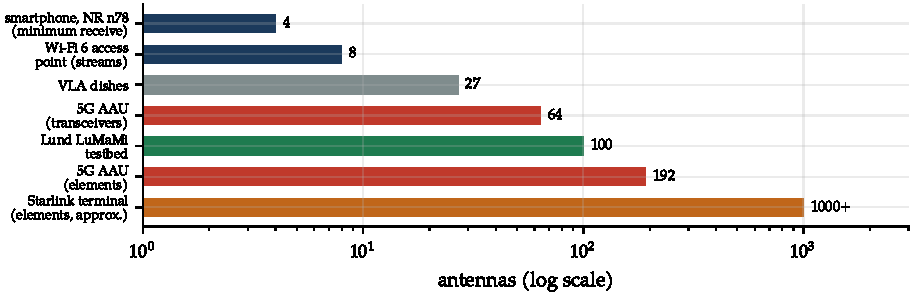
\includegraphics[width=0.92\linewidth]{figs/ch19_by_numbers}\caption{Multi-antenna systems by the numbers (log scale; typical or minimum
values, rounded). From four antennas in a phone to more than a thousand elements in a satellite
terminal, the same mathematics applies.}\label{fig:ch19_by_numbers}\end{figure}

\begin{itemize}
\item Spatial-multiplexing receivers range from ZF (diversity $N_r-N_t+1$) and MMSE through ordered
MMSE-SIC (capacity-achieving with per-stream coding) to ML; sphere and K-best decoders make near-ML
practical, and soft outputs feed the channel decoder.
\item With CSIT, SVD precoding is optimal; FDD systems approximate it with codebooks and RI/PMI/CQI
feedback (LTE, NR Type I and II); limited-feedback theory sets the bits required.
\item Arrays are spatial filters: steering vectors are spatial sinusoids, the beamwidth is about
$101.5^\circ/N$ for half-wavelength spacing, spacing above $\lambda/2$ aliases into grating lobes,
and tapers trade beamwidth for sidelobes. Phase-shifter arrays squint over wide bandwidths; true
time delay does not. Subspace methods such as MUSIC resolve directions beyond the beamwidth.
\item Analog, digital and hybrid architectures trade flexibility against power; millimetre-wave NR
uses hybrid arrays with SSB sweeping and P-1/P-2/P-3 beam management.
\item MU-MIMO serves many users in the same resources: MMSE-SIC on the uplink, DPC as the downlink
ceiling and ZF/RZF linear precoding in practice, with scheduling of nearly orthogonal users.
\item Massive MIMO ($M\gg K$) hardens the channel and makes users nearly orthogonal; TDD reciprocity
with calibration makes channel acquisition scale with $K$, not $M$; pilot contamination limits
simple processing. 64T64R active antennas are now standard 5G macro radios.
\item Cell-free networks, intelligent surfaces, MIMO radar with virtual arrays and LOS MIMO backhaul
apply the same mathematics in new geometries.
\end{itemize}

\begin{labbox}[MIMO: diversity, multiplexing, beamforming and massive MIMO]
Two live labs accompany this chapter:
\begin{itemize}
\item \lab{moderncomms-labs/labs/lab10\_mimo.py}
\item \lab{moderncomms-labs/labs/lab29\_arrays\_beamforming.py}
\end{itemize}
\textbf{Lab~10} has nine experiments: \emph{Fading branches, live} (watch two to eight antennas fade
and the SC, EGC or MRC output ride over the fades); \emph{SC, EGC and MRC error rates} (diversity
order, array gain and the cost of correlation, against Section~\ref{sec:ch19:combining});
\emph{Alamouti versus MRC} (same-symbol transmission, Alamouti, receive MRC and transmit
beamforming, plus a channel that changes between slots); \emph{Eigen-channels and water-filling};
\emph{Ergodic and outage capacity} (i.i.d., correlated and keyhole channels);
\emph{ZF, MMSE, SIC and ML} (live constellations and Monte Carlo error rates); \emph{The
diversity--multiplexing trade-off}; \emph{Massive MIMO: channel hardening} (fade margin, favourable
propagation and pilot contamination); and \emph{MU-MIMO precoding: MR, ZF, RZF} (with beam patterns
for i.i.d.\ and line-of-sight users).
\textbf{Lab~29} takes the array material further: \emph{Steer a line of antennas} (steering,
spacing, grating lobes and tapers); \emph{A planar panel and its EIRP}; \emph{Beam squint: phase vs
true delay}; \emph{Direction finding: MUSIC \& co} (Bartlett, MVDR and MUSIC, coherent sources and
spatial smoothing); \emph{SSB beam sweep and codebook} (NR Type~I beams and PMI loss); \emph{Hybrid
precoding by OMP}; and \emph{Line-of-sight MIMO spacing}. The figure script
\lab{book/figscripts/ch19\_figs.py} generates every data figure in this chapter from the same
\texttt{commlib.mimo} functions, including the sphere decoder, beam squint, MUSIC, limited feedback
and LOS MIMO examples.
\end{labbox}

\problems
\begin{enumerate}[label=\thechapter.\arabic*]
\item Show that the mean output SNR of $L$-branch selection combining in i.i.d.\ Rayleigh fading is
$\bar\gamma\sum_{k=1}^L1/k$. How many branches does selection need to match the mean SNR of
two-branch MRC? Does that make the two schemes equivalent at a BER of $10^{-4}$?
\item Using~\eqref{eq:ch19:chisq}, find the outage probability $P(\gamma<\bar\gamma/10)$ for MRC with
$L=1,2,4$ branches, exactly and with the small-$x$ approximation. How large is $L!$'s effect relative
to selection combining~\eqref{eq:ch19:sccdf}?
\item Two receive antennas see an interferer with channel $\vect{g}=[1,\,e^{j\pi/3}]^{\mathsf T}$ and
power 20\,dB above the noise, and the wanted signal with $\vect{h}=[1,\,-1]^{\mathsf T}$. Compute the
output SINR of MRC and of the optimum combiner~\eqref{eq:ch19:optcomb}. What happens as the two
channel vectors become parallel?
\item For two branches with complex correlation $\rho$, show that MRC is equivalent to combining two
independent branches with mean SNRs $(1\pm|\rho|)\bar\gamma$. Using the high-SNR expansion of the
BER, find the SNR penalty at high SNR as a function of $|\rho|$, and evaluate it for $|\rho|=0.5$ and
$0.9$.
\item Verify that the Alamouti effective channel~\eqref{eq:ch19:alaeff} satisfies
$\vect{H}_{\text{eff}}^{\mathsf H}\vect{H}_{\text{eff}}=(|h_1|^2+|h_2|^2)\vect{I}$, and derive the decoder for
two receive antennas. What happens to the decoder if the channel changes between the two time
slots? Estimate the resulting self-interference for a Doppler of 200\,Hz and a slot of 71\,$\mu$s.
\item Apply the rank criterion to (a) repetition of $s$ from antenna 1 then antenna 2, (b) the
Alamouti code with BPSK, and (c) the scheme that sends $s_1$ and $s_2$ simultaneously from the two
antennas (V-BLAST). What diversity does each achieve with ML decoding and one receive antenna?
\item A $2\times2$ channel is
$\vect{H}=\begin{psmallmatrix}1 & 0.5j\\ 0.3 & -0.8+0.2j\end{psmallmatrix}$. Find its singular values,
the capacity at $\rho=10$\,dB with equal power and with water-filling, and the water level. Below what
SNR does water-filling use only one eigenmode?
\item Show that the ergodic capacity of a $1\times N_r$ SIMO channel grows only as $\log_2(N_r\rho)$
at high SNR, while that of an $N\times N$ channel grows as $N\log_2\rho$. At what SNR does a $4\times4$
channel first have twice the ergodic capacity of a $1\times4$ channel? (Use Figure~\ref{fig:ch19_capacity}
or simulate.)
\item Sketch the optimal DMT for a $3\times2$ channel. Where on it does (a) the Alamouti code with two of
the three antennas, (b) V-BLAST with two streams and ML decoding lie?
\item Derive the post-detection SNR of ZF for stream $k$, $\rho/(N_t[(\vect{H}^{\mathsf H}\vect{H})^{-1}]_{kk})$,
and explain why it has $2(N_r-N_t+1)$ degrees of freedom for i.i.d.\ Rayleigh $\vect{H}$. How many
receive antennas does a ZF receiver need to achieve diversity order 3 with four streams?
\item A 32-element half-wavelength ULA at 3.5\,GHz is steered to $50^\circ$. Find its length, its
half-power beamwidth, the maximum element spacing that avoids grating lobes over $\pm60^\circ$, and the
beam squint at the edges of a 100\,MHz channel. Is squint a concern?
\item An 8T8R FDD base station uses an NR Type I codebook with $N_1=4$, $N_2=1$, two polarisations and
$O_1=4$. How many beams are in the grid? How many bits does a wideband rank-1 PMI need (beam plus
co-phasing)? Compare with the feedback a Type II report would need for $L=4$ beams, 3-bit amplitudes and
8-PSK phases on 13 subbands.
\item A base station with $M=64$ antennas serves $K=8$ users with ZF precoding. Using the result that
the ZF SNR of each user is proportional to a chi-square variable with $2(M-K+1)$ degrees of freedom,
estimate the fraction of power lost to nulling relative to MR, and the 1\% fade margin of each user.
\item \emph{(Simulation)} Extend \texttt{commlib.mmse\_sic\_detect} to produce max-log LLRs and compare
the coded BER (with any rate-1/2 code from Chapter~\ref{ch:classiccodes}) of MMSE, MMSE-SIC and a list
sphere decoder for $4\times4$ 16-QAM.
\item \emph{(Simulation)} Implement hybrid precoding for a 64-element ULA with $N_{\text{RF}}=4$ RF
chains in a sparse channel with five clusters, using orthogonal matching pursuit over a dictionary of
steering vectors. Plot the spectral efficiency against SNR for $N_s=1,2,3$ and compare with
unconstrained SVD precoding.
\item \emph{(Simulation)} Reproduce Figure~\ref{fig:ch19_massive}(b), then add multi-cell MMSE
combining with spatially correlated channels (e.g.\ a one-ring model with a $10^\circ$ angular spread
and users at different angles). Show that the rate no longer saturates.
\end{enumerate}

\furtherreading
\begin{itemize}
\item D.~Tse and P.~Viswanath, \emph{Fundamentals of Wireless Communication}, Cambridge University
Press, 2005. Chapters 3 and 7--10 are the clearest treatment of diversity, the MIMO channel,
capacity, the diversity--multiplexing trade-off and multi-user MIMO; the physical modelling of MIMO
channels in Chapter~7 is outstanding.
\item A.~Paulraj, R.~Nabar and D.~Gore, \emph{Introduction to Space--Time Wireless Communications},
Cambridge University Press, 2003. A compact, rigorous text on MIMO channels, space--time coding and
receivers by one of the inventors.
\item E.~Telatar, ``Capacity of multi-antenna Gaussian channels,'' \emph{European Transactions on
Telecommunications}, vol.~10, no.~6, 1999; and G.~J.~Foschini and M.~J.~Gans, ``On limits of wireless
communications in a fading environment when using multiple antennas,'' \emph{Wireless Personal
Communications}, vol.~6, 1998. The two founding capacity papers.
\item S.~M.~Alamouti, ``A simple transmit diversity technique for wireless communications,''
\emph{IEEE Journal on Selected Areas in Communications}, vol.~16, no.~8, 1998; and V.~Tarokh,
N.~Seshadri and A.~R.~Calderbank, ``Space--time codes for high data rate wireless communication:
performance criterion and code construction,'' \emph{IEEE Transactions on Information Theory},
vol.~44, no.~2, 1998.
\item L.~Zheng and D.~N.~C.~Tse, ``Diversity and multiplexing: a fundamental tradeoff in
multiple-antenna channels,'' \emph{IEEE Transactions on Information Theory}, vol.~49, no.~5, 2003.
\item T.~L.~Marzetta, ``Noncooperative cellular wireless with unlimited numbers of base station
antennas,'' \emph{IEEE Transactions on Wireless Communications}, vol.~9, no.~11, 2010; and
T.~L.~Marzetta, E.~G.~Larsson, H.~Yang and H.~Q.~Ngo, \emph{Fundamentals of Massive MIMO}, Cambridge
University Press, 2016.
\item E.~Bj\"ornson, J.~Hoydis and L.~Sanguinetti, \emph{Massive MIMO Networks: Spectral, Energy, and
Hardware Efficiency}, Foundations and Trends in Signal Processing, 2017 (freely available from the
authors). The most complete modern treatment, with correlated channels, multi-cell MMSE processing
and hardware impairments.
\item R.~W.~Heath Jr.\ and A.~Lozano, \emph{Foundations of MIMO Communication}, Cambridge University
Press, 2018. An engineering-oriented graduate text covering precoding, limited feedback, MU-MIMO
and massive MIMO with care.
\item H.~L.~Van~Trees, \emph{Optimum Array Processing} (Part IV of \emph{Detection, Estimation, and
Modulation Theory}), Wiley, 2002. The encyclopaedic reference on arrays, beam patterns, tapering,
adaptive beamforming and direction finding, including MUSIC and ESPRIT.
\item R.~W.~Heath Jr., N.~Gonz\'alez-Prelcic, S.~Rangan, W.~Roh and A.~M.~Sayeed, ``An overview of
signal processing techniques for millimeter wave MIMO systems,'' \emph{IEEE Journal of Selected Topics
in Signal Processing}, vol.~10, no.~3, 2016. Hybrid architectures, beam training and channel
estimation at millimetre waves.
\item 3GPP TS~38.214 (NR physical-layer procedures for data: CSI reporting, Type I and Type II
codebooks), TS~38.213 (control procedures, SSB and beam failure recovery) and TR~38.901 (channel
models). Dense but definitive; read the codebook sections with this chapter's
Section~\ref{sec:ch19:precoding} beside you.
\end{itemize}
